
\chapter{Control valves}

One of the most common final control elements in industrial control systems is the \textit{control valve}.  A ``control valve'' works to restrict the flow of fluid through a pipe at the command of a remotely sourced signal, such as the signal from a loop controller or logic device (such as a PLC), or even a manual (``hand'') interface controlled by a human operator.  Some control valve designs are intended for discrete (on/off) control of fluid flow, while others are designed to \textit{throttle} fluid flow somewhere between fully open and fully closed (shut), inclusive.  The electrical equivalent of an on/off valve is a switch, while the electrical equivalent of a throttling valve is a variable resistor.  \index{Control valve}  \index{Discrete control valve}  \index{Throttling control valve}  \index{Valves}

Control valves are comprised of two major parts: the \textit{valve body}, containing all the mechanical components necessary to influence fluid flow; and the \textit{valve actuator}, providing the mechanical power necessary to move the valve body components.  Often times, the major difference between an on/off control valve and a throttling control valve is the type of actuator applied to the valve\footnote{To be honest, there are some valve body designs that work far better in on/off service (e.g. ball valves and plug valves) while other designs do a better job at throttling (e.g. double-ported globe valves).  Many valve designs, however, may be pressed into either type of service merely by attaching the appropriate actuator.}: on/off actuators need only position a valve mechanism two one of two extreme positions (fully open or fully closed).  Throttling actuators must be able to accurately position a valve mechanism anywhere between those extremes.   \index{Body, valve} \index{Valve body}  \index{Valve actuator}  \index{Actuator, valve}

Within a control valve body, the specific components performing the work of throttling (or completely shutting off) of fluid flow are collectively referred to as the valve \textit{trim}.  For each major type of control valve, there are usually many variations of trim design.  The choice of valve type, and of specific trim for any type of valve, is a decision dictated by the type of fluid being controlled, the nature of the control action (on/off versus throttling), the process conditions (expected flow rate, temperature, pressures, etc.), and economics.  \index{Trim}  \index{Valve trim}

\vskip 10pt

An appendix of this book (Appendix \ref{valve_tour} beginning on page \pageref{valve_tour}) photographically documents the complete disassembly of a typical control valve.  The valve happens to be a Fisher E-body globe valve with a pneumatic diaphragm actuator.




\filbreak
\section{Sliding-stem valves}

A \textit{sliding-stem} valve body is one where the moving parts slide with a linear motion.  Some examples of sliding-stem valve body designs are shown here:

$$\includegraphics{valve_01.eps}$$ \index{Globe valve} \index{Gate valve} \index{Diaphragm valve}

Most sliding-stem control valves are \textit{direct acting}, which means the valve opens up wider as the stem is drawn out of the body.  Conversely, a direct-acting valve shuts off (closes) when the stem is pushed into the body.  Of course, a \textit{reverse-acting} valve body would behave just the opposite: opening up as the stem is pushed in and closing off as the stem is drawn out.  \index{Direct-acting valve body}  \index{Reverse-acting valve body}



\filbreak
\subsection{Globe valves}

Globe valves restrict the flow of fluid by altering the distance between a movable plug and a stationary seat (in some cases, a pair of plugs and matching seats).  Fluid flows through a hole in the center of the seat, and is more or less restricted by the plug's proximity to that hole.  The globe valve design is one of the most popular sliding-stem valve designs used in throttling service.  A photograph of a small (2 inch) globe valve body appears here:

$$\includegraphics[width=2in]{valve_02.eps}$$

A set of three photographs showing a cut-away Masoneilan model 21000 globe valve body illustrates just how the moving plug and stationary seat work together to throttle flow in a direct-acting globe valve.  The left-hand photo shows the valve body in the fully closed position, while the middle photo shows the valve half-open, and the right-hand photo shows the valve fully open:  \index{Masoneilan model 21000 control valve}

$$\includegraphics[width=1.75in]{valve_10.eps} \hskip 20pt \includegraphics[width=1.75in]{valve_11.eps} \hskip 20pt \includegraphics[width=1.75in]{valve_12.eps} $$

As you can see from these photographs, the valve plug is guided by the stem to maintain alignment with the centerline of the seat.  For this reason, this particular style of globe valve is called a \textit{stem-guided} globe valve.  \index{Stem-guided globe valve}

A variation on the stem-guided globe valve design is the \textit{needle valve}, where the plug is extremely small in diameter and usually fits well into the seat hole rather than merely sitting on top of it.  Needle valves are very common as manually-actuated valves used to control low flow rates of air or oil.  A set of three photographs shows a needle valve in the fully-closed, mid-open, and fully-open positions (left-to-right):  \index{Needle valve}

$$\includegraphics[width=1.75in]{needle_valve_01.eps} \hskip 20pt \includegraphics[width=1.75in]{needle_valve_02.eps} \hskip 20pt \includegraphics[width=1.75in]{needle_valve_03.eps} $$

Yet another variation on the globe valve design is the \textit{port-guided} valve, where the plug has an unusual shape, projecting into the seat.  Thus, the seat ring acts as a guide for the plug to keep the centerlines of the plug and seat always aligned, minimizing guiding stresses that would otherwise be placed on the stem.  This means that the stem may be made smaller in diameter than if the valve trim were stem-guided, minimizing sliding friction and improving control behavior.  \index{Port-guided globe valve}

$$\includegraphics{valve_24.eps}$$

\filbreak

A photograph showing a small port-guided globe valve plug appears in the following photograph:

$$\includegraphics[width=5in]{valve_122.eps}$$

\filbreak

Some globe valves use a pair of plugs (on the same stem) and a matching pair of seats to throttle fluid flow.  These are called \textit{double-ported} globe valves.  The purpose of a double-ported globe valve is to minimize the force applied to the stem by process fluid pressure across the plugs:  \index{Double-ported globe valve}

$$\includegraphics{valve_69.eps}$$

Differential pressure of the process fluid ($P_1 - P_2$) across a valve plug will generate a force parallel to the stem as described by the formula $F = PA$, with $A$ being the plug's effective area presented for the pressure to act upon.  In a single-ported globe valve, there will only be one force generated by the process pressure.  In a double-ported globe valve, there will be \textit{two opposed} force vectors, one generated at the upper plug and another generated at the lower plug.  If the plug areas are approximately equal, then the forces will likewise be approximately equal and therefore nearly cancel.  This makes for a control valve that is easier to actuate (i.e. the stem position is less affected by pressure drop across the valve).

\filbreak

The following photograph shows a disassembled Fisher ``A-body'' double-ported globe valve, with the double plug plainly visible on the right:

$$\includegraphics[width=4in]{valve_70.eps}$$

This particular double-ported globe valve happens to be stem-guided, with bushings guiding the upper stem and also a lower stem (on the bottom side of the valve body).  Double-ported, port-guided control valves also exist, with two sets of port-guided plugs and seats throttling fluid flow.

While double-ported globe valves certainly enjoy the advantage of easier actuation compared to their single-ported cousins, they also suffer from a distinct disadvantage: the near impossibility of tight shut-off.  With \textit{two} plugs needing to come to simultaneous rest on \textit{two} seats to achieve a fluid-tight seal, there is precious little room for error or dimensional instability.  Even if a double-ported valve is prepared in a shop for the best shut-off possible\footnote{The standard preparatory technique is called \textit{lapping}.  To ``lap'' a valve plug and seat assembly, an abrasive paste known as \textit{lapping compound} is applied to the valve plug(s) and seat(s) at the areas of mutual contact when the valve is disassembled.  The valve mechanism is reassembled, and the stem is then rotated in a cyclic motion such that the plug(s) grind into the seat(s), creating a matched fit.  The precision of this fit may be checked by disassembling the valve, cleaning off all remaining lapping compound, applying a metal-staining compound such as \textit{Prussian blue}, then reassembling.  The stem is rotated once more such that the plug(s) will rub against the seat(s), wearing through the applied stain.  Upon disassembly, the worn stain may be inspected to reveal the extend of metal-to-metal contact between the plug(s) and the seat(s).  If the contact area is deemed insufficient, the lapping process may be repeated.}, it may not completely shut off when installed due to dimensional changes caused by process fluid heating or cooling the valve stem and body.  This is especially problematic when the stem is made of a different material than the body.  Globe valve stems are commonly manufactured from stainless steel bar stock, while globe valve bodies are commonly made of cast steel.  Cold-formed stainless steel has a different coefficient of thermal expansion than hot-cast steel, which means the plugs will no longer simultaneously seat once the valve warms or cools much from the temperature it was at when it seated tightly.  \index{Lapping valve plugs and seats}  \index{Prussian blue} 

\filbreak

A more modern version of the globe valve design uses a piston-shaped plug inside a surrounding \textit{cage} with ports cast or machined into it.  These \textit{cage-guided} globe valves throttle flow by uncovering more or less of the port area in the surrounding cage as the plug moves up and down.  The cage also serves to guide the plug so the stem need not be subjected to lateral forces as in a stem-guided valve design.  A photograph of a cut-away control valve shows the appearance of the cage (in this case, with the plug in the fully closed position).  Note the ``T''-shaped ports in the cage, through which fluid flows as the plug moves up and out of the way:  \index{Cage-guided globe valve}

$$\includegraphics[width=4in]{valve_21.eps}$$

An advantage of the cage-guided design is that the valve's flowing characteristics may be easily altered just by replacing the cage with another having different size or shape of holes.  By contrast, stem-guided and port-guided globe valves are characterized by the shape of the plug, which requires further disassembly to replace than the cage in a cage-guided globe valve.  With most cage-guided valves all that is needed to replace the cage is to separate the bonnet from the rest of the valve body, at which point the cage may be lifted out of the body and swapped with another cage.  In order to change a globe valve's plug, you must first separate the bonnet from the rest of the body and then de-couple the plug and plug stem from the actuator stem, being careful not to disturb the packing inside of the bonnet as you do so.  After replacing a plug, the ``bench-set'' of the valve must be re-adjusted to ensure proper seating pressure and stroke calibration.

\filbreak

Cage-guided globe valves are available with both \textit{balanced} and \textit{unbalanced} plugs.  A balanced plug has one or more ports drilled from top to bottom, allowing fluid pressure to equalize on both sides of the plug.  This helps minimize the forces acting on the plug which must be overcome by the actuator:

$$\includegraphics[width=4in]{valve_22.eps}$$

Unbalanced plugs generate a force equal to the product of the differential pressure across the plug and the plug's area ($F = PA$), which may be quite substantial in some applications.  Balanced plugs do not generate this same force because they equalize the pressure on both sides of the plug, however, they exhibit the disadvantage of one more leak path when the valve is in the fully closed position (through the balancing ports, past the piston ring, and out the cage ports):

$$\includegraphics[width=4in]{valve_23.eps}$$

Thus, balanced and unbalanced cage-guided globe valves exhibit similar characteristics to double-ported and single-ported stem- or port-guided globe valves, and for similar reasons.  Balanced cage-guided valves are easy to position, just like double-ported stem-guided and port-guided globe valves.  However, balanced cage-guided valves tend to leak more when in the shut position due to a greater number of leak paths, much the same as with double-ported stem-guided and port-guided globe valves.

\vskip 10pt

\filbreak

Another style of globe valve body is the \textit{three-way} body, sometimes called a \textit{mixing} or a \textit{diverting} valve.  This valve design has three ports on it, with the plug (in this particular case, a cage-guided plug) controlling the degree to which two of the ports connect with the third port:  \index{Three-way globe valve}  \index{3-way globe valve}  \index{Mixing valve}  \index{Diverting valve}

$$\includegraphics{valve_99.eps}$$

This dual illustration shows a three-way valve in its two extreme stem positions.  If the stem is positioned between these two extremes, all three ports will be ``connected'' to varying degrees.  Three-way valves are useful in services where a flow stream must be diverted (split) between two different directions, or where two flow streams must converge (mix) within the valve to form a single flow stream.

\filbreak

A photograph of a three-way globe valve mixing hot and cold water to control temperature is shown here:

$$\includegraphics[height=6in]{valve_100.eps}$$






\filbreak
\subsection{Gate valves}

Gate valves work by inserting a dam (``gate'') into the path of the flow to restrict it, in a manner similar to the action of a sliding door.  Gate valves are more often used for on/off control than for throttling.

The following set of photographs shows a hand-operated gate valve (cut away and painted for use as an instructional tool) in three different positions, from full closed to full open (left to right):

$$\includegraphics[width=1.75in]{gatevalve_closed.eps} \hskip 10pt \includegraphics[width=1.75in]{gatevalve_halfopen.eps} \hskip 10pt \includegraphics[width=1.75in]{gatevalve_open.eps}$$





\filbreak
\subsection{Diaphragm valves}

Diaphragm valves use a flexible sheet pressed close to the edge of a solid dam to narrow the flow path for fluid.  Their operation is not unlike controlling the flow of water through a flexible hose by pinching the hose.  These valves are well suited for flows containing solid particulate matter such as slurries, although precise throttling may be difficult to achieve due to the elasticity of the diaphragm.  The next photograph shows a diaphragm valve actuated by an electric motor, used to control the flow of treated sewage:

$$\includegraphics[width=4in]{valve_03.eps}$$

\filbreak

The following photograph shows a hand-actuated diaphragm valve, the external shape of the valve body revealing the ``dam'' structure against which the flexible diaphragm is pressed to create a leak-tight seal when shut:

$$\includegraphics[width=4in]{valve_121.eps}$$

Some diaphragm valves are pneumatically actuated, using the force of compressed air on one side of the diaphragm to press it against the dam (on the other side) to shut off flow.  This next example is of a small air-actuated diaphragm valve, controlling the flow of water through a 1-inch pipe:

$$\includegraphics[width=4in]{valve_103.eps}$$

The actuating air for this particular diaphragm valve comes through an electric solenoid valve.  The solenoid valve in this photograph has a brass body and a green-painted solenoid coil.






\filbreak
\section{Rotary-stem valves}

A different strategy for controlling the flow of fluid is to insert a rotary element into the flow path.  Instead of sliding a stem into and out of the valve body to actuate a throttling mechanism, rotary valves rely on the rotation of a shaft to actuate the trim.  An important advantage of rotary control valves over sliding-stem designs such as the globe valve and diaphragm valve is a virtually obstructionless path for fluid when the valve is wide-open\footnote{Of course, gate valves also offer obstructionless flow when wide-open, but their poor throttling characteristics give most rotary valve designs the overall advantage.}.

$$\includegraphics{valve_04.eps}$$ \index{Ball valve} \index{Butterfly valve} \index{Disk valve} \index{Eccentric disk valve} \index{High-performance butterfly valve}







\filbreak
\subsection{Ball valves}

In the ball valve design, a spherical ball with a passageway cut through the center rotates to allow fluid more or less access to the passageway.  When the passageway is parallel to the direction of fluid motion, the valve is wide open; when the passageway is aligned perpendicular to the direction of fluid motion, the valve is fully shut (closed).  

The following set of photographs shows a hand-operated ball valve in three different positions, from nearly full closed to nearly full open (left to right):

$$\includegraphics[width=1.75in]{ballvalve_closed.eps} \hskip 10pt \includegraphics[width=1.75in]{ballvalve_halfopen.eps} \hskip 10pt \includegraphics[width=1.75in]{ballvalve_open.eps}$$

Simple ball valves with full-sized bores in the rotating ball are generally better suited for on/off service than for throttling (partially-open) service.  A better design of ball valve for throttling service is the \textit{characterized} or \textit{segmented} ball valve, shown in various stages of opening in the following set of photographs:  \index{Characterized ball valve}  \index{Segmented ball valve}  \index{Ball valve, characterized}  \index{Ball valve, segmented}

$$\includegraphics[height=1.5in]{ballvalve_02.eps} \hskip 10pt \includegraphics[height=1.5in]{ballvalve_03.eps} \hskip 10pt \includegraphics[height=1.5in]{ballvalve_04.eps}$$

The V-shaped notch cut into the opening lip of the ball provides a narrower area for fluid flow at low opening angles, providing more precise flow control than a plain-bore ball valve.






\filbreak
\subsection{Butterfly valves}

Butterfly valves are quite simple to understand: the ``butterfly'' element is a disk that rotates perpendicular to the path of fluid flow.  When parallel to the axis of flow, the disk presents minimal obstruction; when perpendicular to the axis, the disk completely blocks any flow.  Fluid-tight shut-off is difficult to obtain in the classic butterfly design unless the seating area is lined with a soft (elastic) material.







\filbreak
\subsection{Disk valves}

Disk valves (often referred to as \textit{eccentric disk valves}, or as \textit{high-performance butterfly valves}) are a variation on the butterfly design intended to improve seat shut-off.  The disk's center is offset from the shaft centerline, causing it to approach the seat with a ``cam'' action that results in high seating pressure.  Thus, tight shut-off of flow is possible even when using metal seats and disks.

The following photograph shows the body of a Fisher E-plug control valve, with the disk in a partially-open position: \index{Fisher E-plug control valve}

$$\includegraphics[width=4in]{valve_13.eps}$$







\filbreak
\section{Dampers and louvres}

A \textit{damper} (otherwise known as a \textit{louvre}) is a multi-element flow control device generally used to throttle large flows of air at low pressure.  Dampers find common application in furnace and boiler draft control, and in HVAC (Heating, Ventilation, and Air Conditioning) systems.  \index{Damper}  \index{Louvre}  \index{HVAC}

Common damper designs include parallel and radial.  Parallel-vane dampers resemble a Venetian blind, with multiple rectangular vanes synchronously rotated to throttle flow through a rectangular opening.  A photograph of a parallel-vane damper is shown here, part of an induced-draft (suction) air fan system on a separator at a cement plant.  The vanes are not visible in this photograph because they reside inside the metal air duct, but the actuator mechanism and linkages connecting seven vane shafts together are:  \index{Parallel damper}

$$\includegraphics[width=5in]{valve_82.eps}$$

\filbreak

Radial-vane dampers use multiple vanes arranged like petals of a flower to throttle flow through a circular opening.  A photograph of a radial-vane damper is shown here (note the levers and linkages on the periphery of the tube, synchronizing the motions of the eight vanes so they rotate at the same angle):   \index{Radial damper}

$$\includegraphics[width=5in]{valve_05.eps}$$

\filbreak

Dampers find use in many non-industrial applications as well.  Take for instance these greenhouse vents, actuated by pneumatic (air-powered) piston actuators:

$$\includegraphics[width=5in]{valve_25.eps}$$








\filbreak
\section{Valve packing}

Regardless of valve type, all stem-actuated control valves require some form of seal allowing motion of the stem from some external device (an \textit{actuator}) while sealing process fluid so no leaks occur between the moving stem and the body of the valve.  The general term for this sealing mechanism is \textit{packing}.  \index{Packing, valve}  \index{Valve packing}

This mechanical feature is not unlike the \textit{stuffing box} used to seal seawater from entering a boat or ship at the point where the propeller shaft penetrates the hull:

$$\includegraphics{valve_30.eps}$$

The fundamental problem is the same for the ship as it is for the control valve: how to allow a moving shaft to pass through what needs to be an impenetrable barrier to some fluid (in the case of the ship's hull, the fluid is seawater).  The solution is to wrap the shaft in a flexible material that maintains a close fit to the shaft without binding its motion.  A traditional packing material for ship propeller shafts is \textit{flax rope}.  Some form of lubrication is usually provided so this packing material does not impose excessive friction on the shaft's motion\footnote{Some packing materials, most notably Teflon and graphite, tend to be \textit{self-lubricating}.}.  

Modern marine stuffing boxes use advanced materials such as Teflon (PTFE) or graphite instead of flax, which wear longer and leak less water.  In the world of control valves, the traditional packing material used to be asbestos (shaped into rings or ropes, much like flax used to be shaped for use in stuffing boxes), but is now commonly Teflon or graphite as well.

In the case of a ship's stuffing box, a little bit of water leakage is not a problem since all ships are equipped with bilge pumps to pump out collected water over time.  However, leakage is simply unacceptable in many industrial control valve applications where we must minimize \textit{fugitive emissions}.  A ``fugitive emission'' is any unwanted escape of process substance into the surrounding environment, usually from leaks around pump and valve shafts.  Special ``environmental'' packing sets are available for control valve applications where this is a concern.  \index{Fugitive emissions}

\vskip 10pt

\filbreak

Packing in a sliding-stem valve fits in a section of the valve body called the \textit{bonnet}, shown in this simplified diagram of a single-ported, stem-guided globe valve:

$$\includegraphics{valve_32.eps}$$

Here, the packing material takes the form of several concentric rings, stacked on the valve stem like washers on a bolt.  These packing rings are forced down from above by the \textit{packing flange} to apply a compressive force around the circumference of the valve stem.  This compressive force is necessary to generate mechanical stress in the packing material to make it seal tightly against the stem of the valve and the interior wall of the bonnet.

Two nuts threaded onto studs maintain proper force on the packing rings.  Care must be taken not to over-tighten these nuts and over-compress the packing material, or else the packing will create excessive friction on the valve stem.  Not only will this friction impede precise valve stem motion, but it will also create undue wear on the stem and packing, increasing the likelihood of future packing leakage.  Insufficient packing flange force will lead to poor sealing, with process fluid potentially leaking past the packing and out of the valve.

\filbreak

A closer look at the bonnet shows a multitude of components working together to form a low-friction, pressure-tight seal for the moving valve stem:

$$\includegraphics{valve_31.eps}$$

In this diagram, we see two sets of packing rings separated by a metal piece called a \textit{lantern ring}.  The lantern ring acts as a spacer allowing lubricant introduced through the lubrication port to enter into both packing sets from the middle of the bonnet.  \index{Lantern ring}

\vskip 10pt

The packing shown here is ``loaded'' by the compressive force exerted by the packing follower.  The only elasticity in this particular system resides in the packing material itself.  This is called \textit{stationary loading}, otherwise known as \textit{jam} packing.  Over time, as the packing material wears and fatigues, the packing follower must be re-compressed by carefully tightening the packing nuts.   \index{Packing, jam}  \index{Jam packing, valve}  

One must be very careful when torquing the packing nuts on a stationary-loaded packing set.  Insufficient torque (which translates into insufficient stress applied to the packing) will result in process fluid leakage.  Excessive torque (causing excessive stress on the packing) will result in high valve stem friction and premature packing failure.  The latter scenario is what one usually finds in industrial settings, where well-intentioned but uninformed personnel over-tighten valve packing in an effort to prevent leaks.  The proper remedy for a packing assembly that leaks despite having been properly torqued is replacement, not further tightening.

\filbreak

An alternative to ``stationary'' loading is to insert a metal spring into the packing assembly, so that the elasticity of the spring helps to maintain an appropriate amount of packing stress as the packing material wears and ages.  This is called \textit{live loading}, examples of which are shown here:  \index{Live-load packing, valve} \index{Packing, live-loaded}

$$\includegraphics{valve_112.eps}$$

In one of these examples we see a coil spring inside the bonnet used to live-load the packing.  In the other example we see a set of spring-steel washers known as a \textit{Belleville} spring.  Belleville springs have a concave profile, giving them resistance to compression along the shaft axis.  These spring washers are always stacked in opposed pairs (concave against concave, convex against convex) so the washers have room to compress.  \index{Belleville washer spring}

\filbreak

Photographs taken of an actual valve packing assembly removed from the bonnet (left), and re-assembled on the valve stem (right) reveal the structure of the packing and associated components.

$$\includegraphics[width=2.5in]{valve_teardown_13.eps} \hskip 30pt \includegraphics[width=2.5in]{valve_teardown_14.eps}$$

There is no lantern ring in this packing assembly, but there is a coil spring.  This makes it a \textit{live-loaded} packing as opposed to a \textit{jam} packing.  

\filbreak

In packing applications requiring external lubrication, a \textit{stem packing lubricator} may be connected to the lubrication port on the bonnet.  This device uses a long, threaded bolt as a piston to push a quantity grease into the packing assembly:  \index{Valve stem packing lubricator}  \index{Stem packing lubricator}  \index{Packing lubricator}  \index{Lubricator, valve packing}

$$\includegraphics[width=3in]{valve_36.eps}$$

To operate a lubricator, the hand valve on the lubricator is first secured in the closed (shut) position, then the bolt is fully unscrewed until it falls out of the lubricator body.  An appropriate lubricating grease is squeezed into the bolt hole in the lubricator body, and the bolt threaded back into place until hand-tight.  Using a wrench or socket to tighten the bolt a bit more (generating pressure in the grease) and opening the hand valve allows grease to enter the packing chamber.  The bolt is then screwed in fully, pushing the entire quantity of grease into the packing.  As a final step, the hand valve is fully shut so there is no way for process liquid to leak out past the bolt threads.

\vskip 10pt

\filbreak

The two most common packing materials in use today are Teflon (PTFE) and graphite.  Teflon is the better of the two with regard to fluid sealing, stem friction, and stem wear\footnote{Based on friction values shown on page 131 of Fisher's \textit{Control Valve Handbook} (Third Edition), Teflon packing friction is typically 5 to 10 times less than graphite packing for the same stem size!}.  Teflon is also quite resistant to attack from a wide variety of chemical substances.  Unfortunately, it has a limited temperature range and cannot withstand intense nuclear radiation (making it unsuitable for use near reactors in nuclear power plants).  Graphite is another self-lubricating packing material, and it has a far greater temperature range than Teflon\footnote{Graphite packing is usable in services ranging from cryogenic temperatures to 1200 degrees Fahrenheit, as opposed to Teflon which is typically rated between $-40$ $^{o}$F and 450 $^{o}$F.} as well as the ability to withstand harsh nuclear radiation, but creates much more stem friction than Teflon.  Graphite packing also has the unfortunate property of permitting \textit{galvanic corrosion} between the stem and bonnet metals due to its electrical conductivity.  Sacrificial zinc washers are sometimes added to graphic packing assemblies to help mitigate this corrosion, but this only postpones rather than prevents corrosive damage to the stem.  \index{Galvanic corrosion, valve stem packing}  \index{Teflon (PTFE) valve stem packing}  \index{PTFE (Teflon) valve stem packing}   \index{Cryogenic}

The following photographs show samples of woven graphite (left) and Teflon (right) ``rope'' packing, longer pieces of which would normally be found bent around valve stems to form seals.  The graphite packing has a shiny finish and flakes easily, while the Teflon packing is plain white in color and maintains its integrity.  Both feel slippery to the touch:

$$\includegraphics[width=2.5in]{valve_119.eps} \hskip 30pt \includegraphics[width=2.5in]{valve_120.eps}$$

Hybrid packing materials, such as carbon-reinforced Teflon, have been developed in an attempt to combine the best characteristics of both materials.

A legacy valve packing material is \textit{asbestos}, woven into packing rings much the same way as graphite fibers are woven into modern packing rings.  Asbestos is a mineral, which made it suitable for high-temperature process applications.  Its electrical non-conductivity eliminated the galvanic corrosion problem inherent to graphite.  Unfortunately, its classification as a hazardous substance\footnote{Asbestos fibers have the ability to permanently lodge in the air sacs of human lungs, leading to long-term health problems if those fibers are inhaled.} precludes its use as a packing material for contemporary applications.  \index{Asbestos valve stem packing}

\vskip 10pt

\filbreak

A completely different approach to packing is a device called a \textit{bellows seal}: an accordion-like metal tube fastened to the valve stem and to the bonnet, forming a leak-proof seal with negligible friction.  The accordion ribs give the bellows seal an ability to stretch and compress with a sliding stem's linear motion.  Since the bellows is an uninterrupted metal tube, there is no place at all for leaks to develop:  \index{Packing, bellows seal}  \index{Bellows packing seal}

$$\includegraphics{valve_90.eps}$$

The port on the extended bonnet serves as a point of connection for process fluid leak detection sensors, to sound an alarm and/or take action in the event of a ruptured bellows.  The sensor may be as simple as a pressure switch, calibrated to ``trip'' at some modest pressure value below that of the normal process operating pressure.  When the bellows seal breaks\footnote{Bellows have a limited service life, which means the possibility of a rupture is likely.  This is why a conventional packing assembly is always included in a bellows-equipped bonnet.}, the sensor will detect the leak and the standard packing assembly will maintain a reasonable seal until repairs are made on the valve.

\filbreak

An actual bellows seal unit appears in this photograph:

$$\includegraphics[width=5in]{valve86.eps}$$

The accordion-shaped bellows is contained and protected inside the thick metal tube visible in this photograph.  One end of the bellows is welded to the valve stem, and the other end is welded to the protective tube.  With the wide flange of the tube firmly clamped in the bonnet of the valve, a leak-free seal exists.









\filbreak
\section{Valve seat leakage}

In some process applications, it is important that the control valve be able to completely stop fluid flow when placed in the ``closed'' position.  Although this may seem to be a fundamental requirement of any valve, it is not necessarily so.  Many control valves spend most of their operating lives in a partially-open state, rarely opening or closing fully.  Additionally, some control valve designs are notorious for the inability to completely shut off (e.g. double-ported globe valves).  Given the common installation of manual ``block'' valves upstream and downstream of a control valve, there is usually a way to secure zero flow through a pipe even if a control valve is incapable of tight shut-off.  For some applications, however, tight control valve shut-off is mandatory.

For this reason we have several classifications for control valves, rating them in their ability to fully shut off.  Seat leakage tolerances are given roman numeral designations, as shown in this table\footnote{Data in this table taken from Fisher's \textit{Control Valve Handbook}.}:

% No blank lines allowed between lines of an \halign structure!
% I use comments (%) instead, so Tex doesn't choke.

$$\vbox{\offinterlineskip
\halign{\strut
\vrule \quad\hfil # \ \hfil & 
\vrule \quad\hfil # \ \hfil & 
\vrule \quad\hfil # \ \hfil \vrule \cr
\noalign{\hrule}
%
% First row
\textbf{Class} & \textbf{Maximum allowable leakage rate} & \textbf{Test pressure drop} \cr
%
\noalign{\hrule}
%
% Another row
I & (no specification given) & (no specification given) \cr
%
\noalign{\hrule}
%
% Another row
II & 0.5\% of rated flow capacity, air or water & 45-60 PSI or max. operating \cr
%
\noalign{\hrule}
%
% Another row
III & 0.1\% of rated flow capacity, air or water & 45-60 PSI or max. operating \cr
%
\noalign{\hrule}
%
% Another row
IV & 0.01\% of rated flow capacity, air or water & 45-60 PSI or max. operating \cr
%
\noalign{\hrule}
%
% Another row
V & 0.0005 ml/min water per inch orifice size per PSI & Max. operating \cr
%
\noalign{\hrule}
%
% Another row
VI & Bubble test, air or nitrogen & 50 PSI or max. operating \cr
%
\noalign{\hrule}
} % End of \halign 
}$$ % End of \vbox

The ``bubble test'' used for Class VI seat leakage is based on the leakage rate of air or nitrogen gas past the closed valve seat as measured by counting the rate of gas bubbles escaping a bubble tube submerged under water.  For a 6 inch valve, this maximum bubble rate is 27 bubbles per minute (or about 1 bubble every two seconds):

$$\includegraphics{valve_55.eps}$$

It is from this leakage test procedure that the term \textit{bubble-tight shut-off} originates.  Class VI shut-off is often achievable only through the use of ``soft'' seat materials such as Teflon rather than hard metal-to-metal contact between the valve plug and seat.  Of course, this method of achieving bubble-tight shut-off comes at the price of limited operating temperature range and the inability to withstand nuclear radiation exposure.  \index{Bubble-tight valve shut-off}

\vskip 10pt

Special test fixtures are typically used in control valve rebuild shops to test the leakage rates of a rebuilt valve.  One such test bench appears in this photograph:

$$\includegraphics[width=6in]{valve_113.eps}$$

In the foreground of this photograph we see a special ``vise'' used to make quick, pressure-tight connections to the flange of any control valve placed within it.  A movable flange sandwiches the control valve against a stationary flange, both flanges faced with high-density plastic for a pressure-tight fit against the valve body flange faces.  A stainless-steel panel in the background provides a set of air pressure regulators, hand valves, rotameters, pressure gauges, and even a ``bubble'' flow indicator to measure leakage flow rate through the control valve under varying pressure conditions. \index{Rotameter}







\filbreak
\section{Control valve actuators}

The purpose of a control valve \textit{actuator} is to provide the motive force to operate a valve mechanism.  Both sliding-stem and rotary control valves enjoy the same selection of actuators: \textit{pneumatic}, \textit{hydraulic}, \textit{electric motor}, and \textit{hand} (manual).  \index{Actuator}



\filbreak
\subsection{Pneumatic actuators}

Pneumatic actuators use air pressure pushing against either a flexible diaphragm or a piston to move a valve mechanism.  The following photograph shows a cut-away control valve, with a pneumatic diaphragm actuator mounted above the valve body.  You can see the large coil spring providing default positioning of the valve (air pressure acting against the diaphragm moves the valve against the spring) and the rubber diaphragm at the very top.  Air pressure applied to the bottom side of the diaphragm lifts the sliding stem of the valve in the upward direction, against the spring's force which tries to push the stem down:  \index{Pneumatic valve actuator}  \index{Pneumatic diaphragm valve actuator}

$$\includegraphics[width=3in]{valve_07.eps}$$

The amount of force ($F$) in units of pounds generated by any fluid pressing against any surface is equal to the fluid's pressure ($P$) in units of PSI multiplied by the surface area ($A$) in units of square inches ($F = PA$).  In the case of a circular diaphragm, with area equal to $\pi r^2$, the complete formula for force is $F = P \pi r^2$.  For example, a control valve diaphragm 14 inches in diameter (radius = 7 inches) with an applied air pressure of 15 PSI generates a linear force of 2309 pounds.

Air pressure required to motivate a pneumatic actuator may come directly from the output of a pneumatic process controller, or from a \textit{signal transducer} (or \textit{converter}) translating an electrical signal into an air pressure signal.  Such transducers are commonly known as \textit{I/P} or ``I to P'' converters, since they typically translate an electric current signal (I) of 4 to 20 mA DC into an air pressure signal (P) of 3 to 15 PSI. \index{I/P transducer}

\filbreak

The following photographs show I/P transducers of different make and model.  A Fisher model 846 appears in the upper-left photograph, while an older Fisher model 546 appears in the upper-right (with cover removed).  A Foxboro model E69F I/P appears in the lower-left photograph, while a Moore Industries model IPT appears in the lower-right: \index{Fisher model 846 I/P transducer}  \index{Fisher model 546 I/P transducer}  \index{Foxboro model E69F I/P transducer}  \index{Moore Industries model IPT I/P transducer}

$$\includegraphics[width=2.5in]{valve_57.eps} \hskip 30pt \includegraphics[width=2.5in]{valve_58.eps}$$

$$\includegraphics[width=2.5in]{valve_59.eps} \hskip 30pt \includegraphics[width=2.5in]{valve_60.eps}$$

Despite their differing designs and appearances, they all function the same: accepting an analog DC current signal input and a clean supply air pressure of about 20 PSI, outputting a variable air pressure signal proportional to the electric current input.  An interesting feature to compare between these four I/P transducers is their relative ruggedness.  Every transducer shown except the Moore Industries model (lower-right) is built to withstand direct exposure to a process atmosphere, hence the heavy cast-metal housings and electrical conduit fittings.  The Moore Industries unit is intended for a sheltered location, and may be plugged in to a ``manifold'' with several other I/P transducers to form a compact bank of transducers capable of driving air pressure signals to several valve actuators.

\filbreak

Some pneumatic valve actuators are equipped with \textit{handwheels} which are used to manually position the valve in the event of air pressure failure.  The next photograph shows a sliding-stem control valve with pneumatic diaphragm actuator and a ``handwheel'' on the top:  \index{Handwheel, valve}

$$\includegraphics[width=5in]{valve_18.eps}$$

Note the three manual valves located around the control valve: two to \textit{block} flow through the control valve and one to \textit{bypass} flow around the control valve in the event of control valve failure or maintenance.  These manual valves happen to be of the \textit{gate} design, with \textit{rising-stem} actuators to clearly show their status (stem protruding = open valve ; stem hidden = closed valve).  Such block-and-bypass manual valve arrangements are quite common in the process industries where control valves fulfill critical roles and some form of manual control is needed as an emergency alternative.

Note also the air pressure tubing between the valve actuator and the air supply pipe, bent into a loop.  This is called a \textit{vibration loop}, and it exists to minimize strain on the metal tubing from vibration that may occur.  \index{Vibration loop, tubing}

\filbreak

Pneumatic actuators may take the form of pistons rather than diaphragms.  Illustrations of each type are shown here for comparison:

$$\includegraphics{valve_33.eps}$$

Piston actuators generally have longer stroke lengths than diaphragm actuators, and are able to operate on much greater air pressures\footnote{The greater pressure rating of a piston actuator comes from the fact that the only ``soft'' component (the sealing ring) has far less surface area exposed to the high pressure than a rolling diaphragm.  This results in significantly less stress on the elastic ring than there would be on an elastic diaphragm exposed to the same pressure.  There really is no limit to the stroke length of a piston actuator as there is with the stroke length of a diaphragm actuator.  It is possible to build a piston actuator miles long, but such a feat would be impossible for a diaphragm actuator, where the diaphragm must stretch (or roll) the entire stroke length.}.  Since actuator force is a function of fluid pressure and actuator area ($F = PA$), this means piston actuators are able to generate more force than diaphragm actuators of the same diameter.  A 14 inch diaphragm operating at a maximum pressure of 35 PSI generates 5388 pounds of force, but the same size piston operating at a maximum pressure of 150 PSI generates 23091 pounds of force.  The combination of greater force and greater displacement yields more work potential for piston actuators than diaphragm actuators of equivalent size, since mechanical work is the product of force and displacement ($W = Fx$).  

Diaphragm actuators enjoy the definite advantage of less friction than piston actuators.  Less friction means greater precision in positioning the valve stem, which gives diaphragm actuators an advantage over piston actuators where precise valve positioning is important, all other factors being equal.

\filbreak

The following photograph of an ultra-high pressure oxygen valve shows a large pneumatic piston actuating a relatively tiny valve body:

$$\includegraphics[width=5in]{valve_116.eps}$$

Since the only rationale for selecting such a large piston actuator is to generate large actuating force, we may conclude that this relatively small valve body requires an unusually high force to actuate.  This is indeed the case, as the process fluid pressure drop across the valve trim in this application happens to be \textit{several thousand PSI}.  This great of a pressure differential, dropped across even a small valve plug, generates substantial force.  The actuator must generate even more force than this in order to successfully move the valve, and must do so while limited to the typical instrument air pressure value of 100 PSI.  Thus, the only way for the actuator to generate a superior force to the valve plug while working with much less fluid pressure is for the actuator piston to have a much greater area than the plug.

\filbreak

A double-piston pneumatic actuator appears in the next photograph, providing the mechanical force needed to turn an on/off butterfly valve:  \index{Pneumatic piston valve actuator}

$$\includegraphics[width=5in]{valve_08.eps}$$

In this particular actuator design, a pair of pneumatically-actuated pistons move a rack-and-pinion mechanism to convert linear piston motion into rotary shaft motion to move the butterfly trim.  Note the rotary indicator (yellow in color) at the end of the rotary valve stem, showing what position the butterfly valve is in.  Note also the travel switch box (black in color) housing multiple limit switches providing remote indication of valve position to the control room.

\filbreak

A rack-and-pinion mechanism looks like this, as viewed looking into the axis of the rotary shaft:

$$\includegraphics{valve_102.eps}$$

Compressed air applied to the bottom tube (with the top tube vented) pushes both pistons toward the center, spinning the pinion gear counter-clockwise.  Applying compressed air to the top tube (with the bottom tube vented) pushes both pistons outward, rotating the pinion gear clockwise.

\filbreak

An example of this actuator design, cut away to reveal its inner workings, appears here:

$$\includegraphics[width=2.5in]{valve_67.eps} \hskip 30pt \includegraphics[width=2.5in]{valve_68.eps}$$

\filbreak

Another pneumatic piston actuator design uses a simple crank lever instead of a rack-and-pinion gear set to convert linear piston motion into rotary motion.  This next photograph shows such a piston actuator connected to a ball valve:

$$\includegraphics[width=4in]{valve_19.eps}$$

\vskip 10pt

Perhaps the greatest disadvantage of piston actuators as applied to control valves is friction between the piston's pressure-sealing ring and the cylinder wall.  This is not a problem for on/off control valves, but it may be a significant problem for throttling valves where precise positioning is desired.  Diaphragm actuators do not exhibit the same degree of friction as piston actuators because the elastic diaphragm rolls and flexes rather than rubs against a stationary surface as is the case with piston sealing rings.




\filbreak
\subsection{Hydraulic actuators}

Hydraulic actuators use liquid pressure rather than gas pressure to move the valve mechanism.  Nearly all hydraulic actuator designs use a piston rather than a diaphragm to convert fluid pressure into mechanical force.  The high pressure rating of piston actuators lends itself well to typical hydraulic system pressures, and the lubricating nature of hydraulic oil helps to overcome the characteristic friction of piston-type actuators.  Given the high pressure ratings of most hydraulic pistons, it is possible to generate tremendous actuating forces with a hydraulic actuator, even if the piston area is modest.  For example, an hydraulic pressure of 2000 PSI applied to one side of a 3 inch diameter piston will generate a linear thrust exceeding 14000 pounds (7 tons)!

In addition to the ability of hydraulic actuators to easily generate extremely large forces, they also exhibit very \textit{stable} positioning owing to the non-compressibility of hydraulic oil.  Unlike pneumatic actuators, where the actuating fluid (air) is ``elastic,'' the oil inside a hydraulic actuator cylinder does not yield appreciably under stress.  If the passage of oil to and from a hydraulic cylinder is blocked by small valves, the actuator will become firmly ``locked'' into place.  This is an important feature for certain valve-positioning applications where the actuator must firmly hold the valve position in one position.

Some hydraulic actuators contain their own electrically-controlled pumps to provide the fluid power, so the valve is actually controlled by an electric signal.  Other hydraulic actuators rely on a separate fluid power system (pump, reservoir, cooler, hand or solenoid valves, etc.) to provide hydraulic pressure on which to operate.  Hydraulic pressure supply systems, however, tend to be more limited in physical span than pneumatic distribution systems due to the need for thick-walled tubing (to contain the high oil pressure), the need to purge the system of all gas bubbles, and the problem of maintaining a leak-free distribution network.  It is usually not practical to build a hydraulic oil supply and distribution system large enough to cover the entirety of an industrial facility.  Another disadvantage of hydraulic systems compared to pneumatic is lack of intrinsic power storage.  Compressed air systems, by virtue of air's compressibility (elasticity), naturally store energy in any pressurized volumes, and so provide a certain degree of ``reserve'' power in the event that the main compressor shut down.  Hydraulic systems do not naturally exhibit this desirable trait.  \index{Hydraulic valve actuator}

\filbreak

A hydraulic piston actuator attached to a large shut-off valve (used for on/off control rather than throttling) appears in the next photograph.  Two hydraulic cylinders may be seen above the round valve body, mounted horizontally.  Like the pneumatic piston valve shown earlier, this valve actuator uses a rack-and-pinion mechanism to convert the hydraulic pistons' linear motion into rotary motion to turn the valve trim:

$$\includegraphics[width=5in]{valve_06.eps}$$

A feature not evident in this photograph is a hydraulic hand pump that may be used to manually actuate the valve in the event of hydraulic system failure.





\filbreak
\subsection{Self-operated valves}

Although not a type of actuator itself, a form of actuation worthy of mention is where the process fluid pressure itself actuates a valve mechanism.  This self-operating principle may be used in throttling applications or on/off applications, in gas or liquid services alike.  The process fluid may be directly tubed to the actuating element (diaphragm or piston), or passed through a small mechanism called a \textit{pilot} to modulate that pressure before reaching the valve actuator.  This latter design allows the main valve's motion to be controlled by an adjustable device (the pilot).  \index{Pilot-operated control valve}

\filbreak

A very common application for pilot-operated control valves is gas pressure regulation, especially for fuel gas such as propane or natural gas used to fuel large industrial burners.  This next photograph shows a Fisher gas pressure regulator used for regulating the pressure of natural gas fueling an industrial burner:

$$\includegraphics[width=4in]{valve_84.eps}$$

The following diagram shows how a self-operated, spring-loaded gas pressure regulating valve functions:  \index{Spring-loaded pressure regulator}

$$\includegraphics{valve_111.eps}$$

A spring tries to force the plug off the seat, while ``feedback'' gas pressure from the downstream side of the valve acts against a flexible diaphragm to move the plug toward the seat.  The less downstream pressure, the more the trim opens up; the more downstream pressure, the more the trim shuts off.  This spring establishes the pressure-regulating ``setpoint'' value for the regulator.  If a different setpoint is desired, the spring must be replaced with one having a different stiffness.

\filbreak

A variation on this theme is the \textit{pilot-loaded} or \textit{externally-loaded} pressure regulator, using a source of external gas pressure to establish the pressure regulation setpoint.  Here, a simple manual-adjustment pressure regulator serves as the ``pilot'' device to send a loading pressure to the top of the main regulator's actuating diaphragm:  \index{Pilot-loaded pressure regulator}  \index{Externally-loaded pressure regulator}

$$\includegraphics{valve_110.eps}$$

Instead of a stiff internal spring establishing the regulator's pressure setpoint, the externally-supplied loading pressure does that.  Since this loading pressure is easily adjusted by turning the knob on the manual-set pressure regulator, the main regulator now becomes adjustable as well.  The pilot mechanism controls the main gas throttling mechanism, hence the name \textit{pilot}.  \index{Loading pressure}

\filbreak

This next pilot-operated valve is used in a liquid (wastewater) service rather than gas:

$$\includegraphics[width=4in]{valve_85.eps}$$

A consumer-grade application for pilot-operated valves is irrigation system control, where the solenoid valves used to switch water flow on and off to sprinkler heads use pilot mechanisms rather than operate the valve mechanism directly with magnetic force.  A small solenoid valve opens and closes to send water pressure to an actuating diaphragm, which then operates the larger valve mechanism to start and stop the flow of water to the sprinkler.  The use of a pilot allows a relatively small amount of electrical power to control the valve, compared to the amount of electrical power that would be necessary if the solenoid coil were built large enough to actuate the main water valve directly.

\vskip 10pt

A special case of self-operated valve is the \textit{Pressure Relief Valve} (PRV) or \textit{Pressure Safety Valve} (PSV).  These valves are normally shut, opening only when sufficient fluid pressure develops across them to relieve that process fluid pressure and thereby protect the pipes and vessels upstream.  Like the other self-operated valves, these safety valves may directly actuate using process fluid pressure or they may be triggered by a pilot mechanism sending process fluid pressure to the actuator only above certain pressures.  Relief valves using pilots have the advantage of being widely adjustable, whereas non-pilot safety valves usually have limited adjustment ranges.  \index{Pressure Relief Valve (PRV)}  \index{Pressure Safety Valve (PSV)}  \index{PSV}  \index{PRV}  \index{Relief valve}  \index{Safety valve}

For more information on overpressure protection devices (including PRVs and PSVs) refer to section \ref{overpressure_protection} beginning on page \pageref{overpressure_protection}.







\filbreak
\subsection{Electric actuators}

Electric motors have long been used to actuate large valves, especially valves operated as on/off (``shutoff'') devices.  Advances in motor design and motor control circuitry have brought motor-operated valve (MOV) technology to the point where it now competes with legacy actuator technologies such as pneumatic in actuating \textit{throttling} valves as well. \index{MOV}  \index{Motor valve actuator}  \index{Electric motor valve actuator}

Most electric valve actuators use a \textit{worm gear} set to reduce the high rotational speed of the electric motor to a slow rotation suitable for moving a large valve mechanism.  An illustration of a worm gear set appears here:  \index{Worm gear}

$$\includegraphics{valve88.eps}$$

The \textit{worm screw} looks much like a threaded fastener, with its ``threads'' properly pitched to engage with the teeth of the \textit{worm wheel} gear.  As the worm screw turns, it slowly pushes or pulls the circumference of the worm wheel, resulting in a large gear ratio (i.e. many turns of the screw are required to produce a single turn of the wheel).  This slow-turning wheel may then be used to move a sliding-stem valve by means of a threaded shaft (another screw) or used to directly turn a rotary valve (e.g. butterfly, ball, plug).

\filbreak

An electric actuator appears in the next photograph, providing on/off rotary actuation to a ball valve.  This particular electric actuator comes with a hand crank for manual operation, in the event that the electric motor (or the power provided to it) fails:

$$\includegraphics[width=3in]{valve_09.eps}$$

A small lever to the left of the hand crank actuates a \textit{clutch} mechanism to engage or disengage the valve mechanism from the electric motor and the hand wheel.  This clutch ``selects'' either the motor or the hand wheel as the prime mover for the valve, to avoid having the hand wheel spin as the motor turns.  Unless this lever is first moved to the ``manual'' position, turning the hand wheel accomplishes nothing.  \index{Clutch mechanism, electric valve actuator}

\filbreak

The next photograph shows an electric valve actuator coupled to a large butterfly valve.  Although nothing visible in this photograph betrays the nature of this actuator's signaling, it happens to be \textit{digital} rather than analog, receiving position commands through a \textit{Profibus} digital network rather than an analog 4-20 mA current signal:  \index{Rotork electric valve actuator}

$$\includegraphics[width=5in]{valve_83.eps}$$

The shape of the actuator's metal casing reveals the final gear drive of this actuator as a \textit{worm gear} set.  Note the round shape of the casing where the open/close indicator is located (at the centerline of the butterfly valve stem): this contains the worm wheel.  Note immediately to the left of that round casing is a vertically-oriented cylinder shape: this contains the worm screw, which engages with the teeth of the worm wheel.  Above the worm screw is a parallel-shaft \textit{spur gear} set which acts to further reduce the speed of the actuator's electric motor: the motor shaft terminates in a small gear, which meshes with a larger gear that turns the worm screw shaft.  Above the parallel-shaft gear set is the main casing of the actuator, which actually contains its own internal worm gear set.  This multiple-stage gear reduction means that the motor spins very fast in comparison to the butterfly element inside the valve, and that the butterfly is capable of exerting a fantastic amount of torque in comparison to the torque rating of the electric motor.  \index{Worm gear}  \index{Gear, worm}  \index{Gear, spur}  \index{Spur gear}

\vskip 10pt

Electric motors require no external fluid power system to function, unlike pneumatic or hydraulic actuators.  All they require is a source of electrical power (often 480 volts AC, three-phase).  Some electric valve actuators even have the capability of operating from the power of an electric battery pack, for reliable operation in the event of a power system outage.

Virtually all electric valve actuators require some form of \textit{feedback} to indicate the valve's position.  At minimum, this consists of \textit{limit switches} to indicate when the valve is fully shut and fully open.  For throttling services, an electric actuator requires an actual valve position sensor so that it may precisely adjust the valve to any desired state.  This sensor may take the form of a potentiometer, or a variable differential transformer (LVDT or RVDT), or pulse encoder. \index{LVDT}  \index{RVDT}

\filbreak

This Rotork brand MOV has a digital display at one end showing its closed status both in text (``Closed Limit'') and symbolically (by the vertical line, which is supposed to represent a closed butterfly element):

$$\includegraphics[width=4in]{valve_97.eps}$$

In addition to visual indicators of status, electric valve actuators commonly provide auxiliary electrical contacts signaling fully-open and fully-closed positions, which may be used to energize remote indicator lights or discrete input channels of control systems (e.g. PLC).  Throttling-service MOVs also provide analog (and/or digital) signaling of valve stem position for remote indication or feedback to an electronic control system.





\filbreak
\subsection{Hand (manual) actuators}

Valves may also be actuated by hand power alone.  The following valves are all ``manual'' valves, requiring the intervention of a human operator to actuate: \index{Hand valve actuator}  \index{Manual valve actuator}

$$\includegraphics[width=2.5in]{valve_14.eps} \hskip30pt \includegraphics[width=2.5in]{valve_15.eps}$$

$$\includegraphics[width=2.5in]{valve_16.eps} \hskip30pt \includegraphics[width=2.5in]{valve_17.eps}$$

Note the threaded stem of the lower-left valve.  This stem rises and falls with the handle's turning, providing visual indication of the valve's status.  Such an actuator is called a \textit{rising-stem} design.  Also note the chain on the upper-right actuator wheel, allowing operation of the high-mounted valve from a ground-level position.  \index{Rising stem valve actuator}

\vskip 10pt

\filbreak

A hybrid of hand and pneumatic valve actuation is seen on this Valtek brand control valve, where the control valve assembly is actuated by a pneumatic piston actuator, but is also equipped with a manually-operated ``handwheel'':  \index{Handwheel, control valve}

$$\includegraphics[height=3in]{valve_124.eps}$$

A handwheel mechanism may be used to override the pneumatic actuator simply by overpowering it in either direction (i.e. providing a greater force on the valve stem than the piston actuator provides) or it may be left in a neutral position to allow the pneumatic actuator full control over valve stem position.  Handwheels may be used to override the control valve's pneumatic actuator to either the full-open or full-closed positions, or it may simply be used to assert a high- or low-limit ``stop'' to the valve stem to prohibit stem motion beyond a certain position.

Note the ``lockout'' tab flipped to the horizontal position near the handwheel, located between two of the handwheel's spokes.  This simple mechanism permits the handwheel to be locked out to prevent accidental turning.









\filbreak
\section{Valve failure mode}

An important design parameter of a control valve is the position it will ``fail'' to if it loses motive power.  For electrically actuated valves, this is typically the last position the valve was in before loss of electric power.  For pneumatic and hydraulic actuated valves, the option exists of having a large spring provide a known ``fail-safe'' position (either open or closed) in the event of fluid pressure (pneumatic air pressure or hydraulic oil pressure) loss.  \index{Fail-safe mode for a control valve}






\filbreak
\subsection{Direct/reverse actions}

The fail-safe mode of a pneumatic/spring valve is a function of both the actuator's action and the valve body's action.  For sliding-stem valves, a \textit{direct-acting} actuator pushes down on the stem with increasing pressure while a \textit{reverse-acting} actuator pulls up on the stem with increasing pressure.  Sliding-stem valve bodies are classified as \textit{direct-acting} if they open up when the stem is lifted, and classified as \textit{reverse-acting} if they shut off (close) when the stem is lifted.  Thus, a sliding-stem, pneumatically actuated control valve may be made \textit{air-to-open} or \textit{air-to-close} simply by matching the appropriate actuator and body types.  

\filbreak

The most common combinations mix a direct-acting valve body with either a reverse- or direct-acting valve actuator, as shown in this illustration:  \index{Air-to-open valve}  \index{Air-to-close valve}  \index{Direct valve actuator}  \index{Reverse valve actuator}  \index{Direct valve body}

$$\includegraphics{valve_20.eps}$$

\filbreak

Reverse-acting valve bodies may also be used, with opposite results:  \index{Reverse valve body}

$$\includegraphics{valve_91.eps}$$

The reverse-acting gate valve body shown in the left-hand illustration is open, with fluid flowing \textit{around} the stem while the wide plug sits well below the seat area.  Reverse-acting valve bodies tend to be more complex in construction than direct-acting valve bodies, and so they are less common in control valve applications.  An interesting exception to this trend -- although not technically a \textit{control} valve but rather a self-actuated device -- is the Fisher model 1098EGR pilot-operated pressure regulator which uses a reverse-acting valve body to throttle the flow of gas through it.  \index{Fisher model 1098EGR pilot-operated pressure regulator}






\filbreak
\subsection{Available failure modes}

Valve fail mode may be shown in instrument diagrams by either an arrow pointing in the direction of failure (assuming a direct-acting valve body where stem motion toward the body closes and stem motion away from the body opens the valve trim) and/or the abbreviations ``FC'' (fail closed) and ``FO'' (fail open).  Other failure modes are possible, as indicated by this set of valve symbols:  \index{Fail open}  \index{Fail closed}

$$\includegraphics{diagrams05.eps}$$

In order for a pneumatic or hydraulic valve to fail in the \textit{locked} state, an external device must trap fluid pressure in the actuator's diaphragm or piston chamber in the event of supply pressure loss.  \index{Fail locked}

Valves that fail in place and drift in a particular direction are usually actuated by double-acting pneumatic piston actuators.  These actuators do not use a spring to provide a definite fail mode, but rather use air pressure both to open and to close the valve.  In the event of an air pressure loss, the actuator will neither be able to open nor close the valve, and so it will tend to remain in position.  If the valve is of the globe design with unbalanced trim, forces exerted on the valve plug will move it in one direction (causing drift).







\filbreak
\subsection{Selecting the proper failure mode}

It is important to note how the failure mode of a valve is often linked to its control action (air-to-open, air-to-close)\footnote{Exceptions exist for valves designed to fail in place, where a valve may be engineered to ``lock'' in position through the action of an external device whether the valve itself is air-to-open or air-to-close.}.  That is, an air-to-open pneumatic control valve will fail closed on loss of air pressure, and vice-versa.  This is an important fact because good safety engineering demands that the risk factors of the process determine proper valve failure mode rather than control system convention or habit.  People may find it easier to understand the operation of an air-to-open control valve than an air-to-close valve (more signal = more process fluid flow), but this should not be a guiding principle in valve selection.  Air-to-open control valves naturally fail closed which means they are appropriate for a particular process control application \textit{only} if that process is safer with a failed-closed valve than with a failed-open valve.  If the process is safer with a fail-open valve, then the pneumatically-actuated control valve specified for that application needs to be air-to-close.

\label{failsafe_design}

In fact, this basic principle forms the basis -- or at least it \textit{should} form the basis -- of decisions made for all instrument actions in critical control loops: first determine the safest mode of valve failure, then select and/or configure instrument actions in such a way that the most probable modes of signal path failure will result in the control valve consistently moving to that (safest) position.

For example, consider this automated cooling system for a large power-generating engine:

$$\includegraphics{valve59.eps}$$

Clearly, it is more hazardous to the engine for the valve to fail closed than it would be for the valve to fail open.  If the valve fails closed, the engine will surely overheat from lack of cooling.  If it fails open, the engine will merely run cooler than designed, the only negative consequence being decreased efficiency.  With this in mind, the only sensible choice for a control valve is one that fails open (air-to-close).

However, our choices in instrument action do not end with the control valve.  How should the temperature transmitter, the controller, and the I/P transducer be configured to act?  In each case, the answer should be to act in such a way that the valve will default to its fail-safe position (wide open) in the event of the most likely input signal fault.

Stepping ``backward'' through the control system from the valve to the temperature sensor, the next instrument we encounter is the I/P transducer.  Its job, of course, is to convert a 4-20 mA current signal into a corresponding pneumatic pressure that the valve actuator can use.  Since we know that the valve's failure mode is based on a loss of actuating air pressure, we want the I/P to be configured in such a way that it outputs minimum pressure in the event of an electrical fault in its 4-20 mA input signal wiring.  Whether the wiring fails shorted or fails open, the result will be 0 milliamps at the I/P input terminals.  Thus, the configuration of the I/P transducer should be \textit{direct}, such that a 4 to 20 mA input signal produces a 3 to 15 PSI output pressure, respectively (i.e. minimum input current yields minimum output pressure).

The next instrument in the loop is the controller.  Here, we want the most likely input signal failure to result in a minimum output signal, so the valve will (once again) default to its ``fail safe'' position.  Consequently, we should configure the controller for \textit{direct} action just like we did with the I/P transducer (i.e. a decreasing PV signal from a broken wire or loose connection in the input circuit results in a decreasing output signal).

Finally, we come to the last instrument in the control loop: the temperature transmitter (TT).  As with most instruments, we have the option of configuring it for direct or reverse action.  Should we choose direct (i.e. hotter engine = more mA output) or reverse (hotter engine = less mA output)?  Here, our choice needs to be made in such a way that the overall effect of the control system is \textit{negative feedback}.  In other words, we need to configure the transmitter such that a hotter engine results in increased coolant flow (a wider-open control valve).  Since we know the rest of the system has been designed so a minimum signal anywhere tends to drive the valve to its fail-safe mode (wide open), we must choose a \textit{reverse-acting} transmitter, so a hotter engine results in a decreased milliamp signal from the transmitter.  If the transmitter has a sensor ``burnout'' mode switch, we should flip this switch into the low-scale burnout position, so a burned-out sensor will result in 4 mA output (low end of the 4-20 mA scale), thus driving the valve into its safest (wide-open) position.  \index{Negative feedback}

Such a configuration -- with its air-to-close control valve and a reverse-acting transmitter -- may seem strange and counter-intuitive, but it is the safest design for this engine cooling system.  We arrived at this ``odd'' configuration of instruments by first choosing the safest control valve failure mode, then choosing instrument actions in such a way that the most likely signal-path failures anywhere in the system would result in the same, consistent valve response.  Of course it should go without saying that accurate documentation in the form of a loop diagram with instrument actions clearly shown is an absolutely essential piece of the whole system.  If the safety of a control system depends on using any ``non-standard'' instrument configurations, those configurations had better be documented so those maintaining the system in the future will know what to expect!

\vskip 10pt

Another important detail in this system is to configure the controller such that the operator display for the output signal still registers in an intuitive way: 0\% should still represent a shut control valve, while 100\% should still represent a wide-open valve.  With the valve being air-to-close (signal-to-close from the controller's perspective), this means the controller should be configured for \textit{reverse indication}\footnote{Note that reverse \textit{indication} is not the same thing as reverse \textit{action} for a loop controller.  Reverse indication simply means the output display shows 100\% valve position at 4 mA output, and 0\% valve position at 20 mA output.  Reverse action means the output decreases when the input (process variable) increases.} on the output display, so that an output of 4 mA (wide-open valve) reads 100\% open, and an output of 20 mA (fully shut valve) reads 0\%.  As confusing as this might be for the technician who must service the controller, it is more important that the operator using this controller every working day sees something that makes intuitive sense.  ``Minor'' details such as this become critically important if an emergency ever occurs, and the operator must make split-second decisions based on the indications they see!  \index{Reverse indication, controller output}













\filbreak
\section{Actuator bench-set}

Valve actuators provide force to move control valve trim.  For precise positioning of a control valve, there must be a calibrated relationship between applied force and valve position.  Most pneumatic actuators exploit \textit{Hooke's Law} to translate applied air pressure to valve stem position.   \index{Hooke's Law}

$$F = kx$$

\noindent
Where,

$F$ = Force applied to spring in newtons (metric) or pounds (British)

$k$ = Constant of elasticity, or ``spring constant'' in newtons per meter (metric) or pounds per foot (British)

$x$ = Displacement of spring in meters (metric) or feet (British)

\vskip 10pt

Hooke's Law is a linear function, which means that spring motion will be linearly related to applied force from the actuator element (piston or diaphragm).  Since the working area of a piston or diaphragm is constant, the relationship between actuating fluid pressure and force will be a simple proportion ($F = PA$).  By algebraic substitution, we may alter Hooke's Law to include pressure and area:

$$F = kx$$

$$PA = kx$$

\filbreak

Solving for spring compression as a function of pressure, area, and spring constant:

$$x = {PA \over k}$$

$$\includegraphics{valve_26.eps}$$

When a control valve is assembled from an actuator and a valve body, the two mechanisms must be coupled together in such a way that the valve moves between its fully closed and fully open positions with an expected range of air pressures.  A common standard for pneumatic control valve actuators is 3 to 15 PSI\footnote{3 PSI could mean fully closed and 15 PSI fully open, or vice-versa, depending on what form of actuator is coupled to what form of valve body.  A direct-acting actuator coupled to a direct-acting valve body will be open at low pressure and closed at high pressure (increasing pressure pushing the valve stem toward the body, closing off the valve trim), resulting in \textit{air-to-close} action.  Reversing either actuator or valve type (e.g. reverse actuator with direct valve or direct actuator with reverse valve) will result in \textit{air-to-open} action.}.

There are really only two mechanical adjustments that need to be made when coupling a pneumatic diaphragm actuator to a sliding-stem valve: the \textit{stem connector} and the \textit{spring adjuster}.  The stem connector mechanically joins the sliding stems of both actuator and valve body so they move together as one stem.  This connector must be adjusted so neither the actuator nor the valve trim prevents full travel of the valve trim:  \index{Stem connector, control valve}  \index{Spring adjuster, valve actuator}

$$\includegraphics{valve_27.eps}$$

Note how the plug rests fully on the seat when the valve is closed, and how the travel indicator indicates fully open at the point where the actuator diaphragm nears its fully upward travel limit.  This is how things should be when the stem connector is properly adjusted.

\filbreak

If the stem connector is set with the actuator and valve stems spaced too far apart (i.e. the total stem length is too long), the actuator diaphragm will bind travel at the upper end and the valve plug will bind travel at the lower end.  The result is a valve that cannot ever fully open:

$$\includegraphics{valve_29.eps}$$

A control valve improperly adjusted in this manner will never achieve full-flow capacity, which may have an adverse impact on control system performance.

\filbreak

If the stem connector is set with the actuator and valve stems too closely coupled (i.e. the total stem length is too short), the actuator diaphragm will bind travel at the lower end and the valve plug will bind travel at the upper end.  The result is a valve that cannot ever fully close:

$$\includegraphics{valve_28.eps}$$

This is a very dangerous condition: a control valve that lacks the ability to fully shut off.  The process in which this valve is installed may be placed in jeopardy if the valve lacks the ability to stop the flow of fluid through it!

\vskip 10pt

Once the stem length has been properly set by adjusting the stem connector, the spring adjuster must be set for the proper \textit{bench set} pressure.  This is the pneumatic signal pressure required to lift the plug off the seat.  For an air-to-open control valve with a 3 to 15 PSI signal range, the ``bench set'' pressure would be 3 PSI.  \index{Bench set, control valve}

Bench set is a very important parameter for a control valve because it establishes the seating force (\textit{seat load}) of the plug against the seat when the valve is fully closed.  Proper seating pressure is critical for tight shut-off, which carries safety implications in some process services.  Consult the manufacturer's instructions when adjusting the bench set pressure for any sliding-stem control valve.  These instructions will typically guide you through both the stem connector and the spring adjuster procedures, to ensure both parameters are correctly set.  \index{Seat load, control valve}








\filbreak
\section{Pneumatic actuator response}

A limitation inherent to pneumatic valve actuators is the amount of air flow required to or from the actuator to cause rapid valve motion.  This is an especially acute problem in all-pneumatic control systems, where the distance separating a control valve from the controller may be substantial:

$$\includegraphics{valve_61.eps}$$

The combined effect of air-flow friction in the tube, flow limitations inherent to the controller mechanism, and volume inside the valve actuator conspire to create a sluggish valve response to sudden changes in controller output signal, not unlike the response of an RC (resistor-capacitor) time-delay circuit where a step-change in voltage input results in an inverse exponential output signal. 

\filbreak

If the pneumatic valve actuator is driven by an I/P transducer instead of directly by a pneumatic controller, the problem is lessened by the ability to locate the I/P close to the actuator, thus greatly minimizing tube friction and thus minimizing the ``time constant'' ($\tau$) of the control valve's response:

$$\includegraphics{valve_62.eps}$$

Still, if the pneumatic actuator is particularly large in volume, an I/P transducer may experience trouble supplying the necessary air flow rate to rapidly actuate the control valve.  Certainly the problem of time delay is reduced, but not eliminated, by the close-coupled location of the I/P transducer to the actuator.

\vskip 10pt

One way to improve valve response in either type of system (full-pneumatic or I/P-driven) is to use a device known as a \textit{volume booster} to source and vent compressed air for the valve actuator.  A ``volume booster'' is a pneumatic device designed to reproduce a pneumatic pressure signal (1:1 ratio), but with far greater output flow capacity.  In electrical terms, a volume booster is analogous to a \textit{voltage follower}: a circuit designed to boost current to a load, without boosting or diminishing voltage.  A 3 to 15 PSI pneumatic pressure signal applied to the input of a volume booster will result in an identical output signal (3 to 15 PSI), but with greatly enhanced flow capacity.  

\filbreak

A pneumatic control system equipped with a volume booster would look something like this: \index{Volume booster}

$$\includegraphics{valve_63.eps}$$

Of course, enhanced air flow to and from the actuator does not completely eliminate time delays in valve response.  So long as the flow rate into or out of an actuator is finite, some time will be required to change pressure inside the actuator and thus change valve position.  However, if the actuator volume cannot be reduced for practical reasons of actuating force (larger diaphragm or piston area needed for more force, also resulting in more volume for any given stroke length), then the only variable capable of reducing time lag is increased air flow rate, and a volume booster directly addresses that deficiency.

\filbreak

Internally, a volume booster's construction is not unlike a manually-adjusted pressure regulator\footnote{The volume booster design shown here is loosely based on the Fisher model 2625 volume boosting relay.}:  \index{Fisher model 2625 volume boosting relay}

$$\includegraphics{valve_64.eps}$$

In either mechanism, an internal diaphragm senses output pressure and acts against a restraining force (either a spring preloaded by a hand adjustment screw or an external pressure signal acting on another diaphragm) to position an air flow throttling/venting mechanism.  If the output pressure is less than desired, the diaphragm moves down to open the air sourcing plug and supply additional air volume to the output.  If the output pressure is greater than desired, the diaphragm moves up to shut off the sourcing plug and open up the venting port to relieve air pressure to atmosphere.









\filbreak
\section{Valve positioners}

The reason why a pneumatic control valve's stem position corresponds linearly to the amount of air pressure applied to the actuator is because mechanical springs tend to follow \textit{Hooke's Law}, where the amount of spring motion ($x$) is directly proportional to applied force ($F = kx$).  A pneumatic actuator applies force as a function of air pressure and piston/diaphragm area ($F = PA$), and the spring in turn compresses or stretches to generate an equal and opposite reaction force.  The end-result is that actuator pressure linearly translates into valve stem motion ($x = {PA \over k}$).   \index{Hooke's Law}

This linear and repeatable relationship between pneumatic signal pressure and valve stem position holds true if and only if the actuating diaphragm/piston and spring are the sole forces at work on the valve stem.  If any \textit{other} force acts upon this mechanism, the relationship between signal pressure and valve stem position will no longer be ideal.

Unfortunately, there exist many other forces acting on a valve stem besides the actuator force and the spring's reaction force.  Friction from the stem packing is one such force, and reaction force at the valve plug caused by differential pressure across the plug's area is another\footnote{One way to minimize dynamic forces on a globe valve plug is to use a \textit{double-ported} plug design, or to use a \textit{balanced} plug on a cage-guided globe valve.  A disadvantage to both these valve plug designs, though, is greater difficulty achieving tight shut-off.}.  These forces conspire to re-position the valve stem so stem travel does not precisely correlate to actuating fluid pressure.

A common solution to this dilemma is to add a \textit{positioner} to the control valve assembly.  A positioner is a motion-control device designed to actively compare stem position against the control signal, adjusting pressure to the actuator diaphragm or piston until the correct stem position is reached:

$$\includegraphics{valve_56.eps}$$

Positioners essentially act as control systems within themselves\footnote{The technical term for this type of control system is \textit{cascade}, where one controller's output becomes the setpoint for a different controller.  In the case of a valve positioner, the positioner receives a valve stem position setpoint from the main process controller.  We could say that the main process controller in this case is the \textit{primary} or \textit{master} controller, while the valve positioner is the \textit{secondary} or \textit{slave} controller.}: the valve's stem position is the process variable (PV), the command signal to the positioner is the setpoint (SP), and the positioner's signal to the valve actuator is the manipulated variable (MV) or output.  Thus, when a process controller sends a command signal to a valve equipped with a positioner, the positioner receives that command signal and applies as much or as little air pressure to the actuator as needed in order to achieve that desired stem position.  Thus, the positioner will ``fight'' against any other forces acting on the valve stem to achieve crisp and accurate stem positioning according to the command signal.  A properly functioning positioner ensures the control valve will be ``well-behaved'' and obedient to the command signal.

\filbreak

The following photograph shows a Fisher model 3582 pneumatic positioner mounted to a control valve.  The positioner is the grey-colored box with three pressure gauges on its right-hand side:  \index{Fisher model 3582 valve positioner}

$$\includegraphics[width=3in]{valve_34.eps}$$

On the left-hand side of this positioner may be seen part of the feedback mechanism: a metal bracket bolted to the valve stem connector, linking to an arm coming out of the positioner's side.  Every control valve positioner must be equipped with some means to sense the position of the valve's stem, otherwise the positioner could not compare the valve stem's position against the command signal.

\filbreak

A more modern positioner appears in the next photograph, the Fisher DVC6000 (again, the grey-colored box with pressure gauges on its right-hand side):  \index{Fisher model DVC6000 valve positioner}

$$\includegraphics[width=3in]{valve_35.eps}$$

Like the older model 3582 positioner, this DVC6000 model uses a feedback linkage on the left-hand side to sense the valve stem's position.  The even newer model DVC6200 uses a magnetic \textit{Hall Effect} sensor to sense the position of a magnet bolted to the valve stem.  This non-mechanical position feedback design eliminates backlash, wear, interference, and other potential problems associated with mechanical links.  Better feedback is essential to better valve positioning.  \index{Fisher model DVC6200 valve positioner} \index{Hall Effect sensor}

\vskip 10pt

Control valve positioners are typically constructed in such a way to source and vent high air flow rates, such that the positioner also fulfills the functionality of a volume booster\footnote{This is not to say valve positioners have no need for external volume boosters, just that the actuating air flow capacity of a typical positioner greatly exceeds the air flow capacity of a typical I/P transducer.}.  Thus, a positioner not only ensures more precise valve stem positioning, but also faster stem velocity (and shorter time delays) than if the valve actuator were directly ``powered'' by an I/P transducer.

\filbreak

Another advantage of adding a positioner to a pneumatically actuated control valve is superior valve seating (tight shutoff).  This benefit is not obvious at first inspection, and so some explanation is in order.  

First, one must understand that mere contact between the plug and seat within a sliding-stem valve is not enough to ensure tight shut-off.  Rather, the plug must be \textit{forcefully} pressed down onto the seat in order to fully shut off all flow through the valve.  Anyone who has ever tightened the handle on a leaking hose bib (garden spigot) intuitively understands this principle: a certain amount of contact force between the plug and the seat is necessary in order to slightly deform and thereby mold those two components to a perfect fluid-tight fit.  The technical term for this mechanical requirement is \textit{seat load}.   \index{Seat load, control valve}

Imagine if you will a diaphragm-actuated, sliding-stem, air-to-open control valve with a bench set range of 3 to 15 PSI.  At an applied actuator pressure of 3 PSI, the diaphragm generates just enough force to exactly overcome the actuator spring's pre-load force, but not enough force to actually move the plug off the seat.  In other words, at 3 PSI diaphragm pressure, the plug is touching the seat but with little or no force to provide a tight shut-off seal.  If this control valve is directly powered by an I/P transducer with a 3-15 PSI calibrated range, it means the valve will be barely shut at a 0\% signal value (3 PSI) rather than tightly shut off.  In order to fully force the valve plug against the valve seat to achieve a tight seal, \textit{all} air pressure would have to be vented from the diaphragm to ensure no diaphragm force opposing the spring.  This is impossible with an I/P having a calibrated range of 3-15 PSI.

Now imagine that exact same valve equipped with a positioner, taking the 3-15 PSI signal from the I/P and using it as a command (setpoint) for valve stem position, applying as much or as little pressure to the diaphragm as necessary to achieve the desired stem position.  Proper positioner calibration is such that the valve stem does not begin to lift until the signal has risen slightly \textit{above} 0\%, which means at 0\% (4 mA) the positioner will be trying to force the valve to a slightly \textit{negative} stem position.  In attempting to achieve this impossible demand, the positioner's output will saturate low, applying no pressure whatsoever to the actuating diaphragm, resulting in full spring force applied by the plug against the seat.  A comparison of the two scenarios is shown here:

$$\includegraphics{valve_114.eps}$$

\vskip 10pt

While positioners are beneficial on spring-equipped valve actuators, they are absolutely essential for some other styles of actuators.  Consider the following double-acting pneumatic piston actuator which has no spring:

$$\includegraphics{valve_115.eps}$$

Without a spring providing a restraining force to return the valve to a ``fail-safe'' position, there exists no Hooke's Law relationship between applied air pressure and stem position.  A positioner must alternately apply air pressure to \textit{both} surfaces of the piston to raise and lower the valve stem.

Electric control valve actuators are another class of actuator design absolutely requiring some form of positioner system, because an electric motor is not ``aware'' of its own shaft position in order that it may precisely move a control valve.  Thus, a positioner circuit using a potentiometer or LVDT/RVDT sensor to detect valve stem position and a set of transistor outputs to drive the motor is necessary to make an electric actuator responsive to an analog control signal. \index{LVDT}  \index{RVDT} 






\filbreak
\subsection{Force-balance pneumatic positioners}

A simple force-balance pneumatic valve positioner design appears in the following cutaway illustration:  \index{Force-balance valve positioner}

$$\includegraphics{valve_37.eps}$$

The control signal for this valve is a 3 to 15 PSI pneumatic signal, coming from either an I/P transducer or a pneumatic controller (neither one shown in the illustration).  This control signal pressure applies an upward force on the force beam, such that the baffle tries to approach the nozzle.  Increasing backpressure in the nozzle causes the pneumatic amplifying relay to output a greater air pressure to the valve actuator, which in turn lifts the valve stem up (opening up the valve).  As the valve stem lifts up, the spring connecting the force beam to the valve stem becomes further stretched, applying additional force to the right-hand side of the force beam.  When this additional force balances the bellows' force, the system stabilizes at a new equilibrium.

Like all force-balance systems, the force beam motion is constrained by the balancing forces, such that its motion is negligible for all practical purposes.  In the end, equilibrium is achieved by one force balancing another, like two teams of people pulling oppositely on a length of rope\footnote{In an earlier chapter of this book, force- and motion-balance pneumatic mechanisms were likened to ``tug-of-war'' contestants versus ballroom dancers, respectively.  Force-balance mechanisms pit force against force to achieve mechanical balance, like two teams competing in a tug-of-war where opposing forces are perfectly balanced and no motion takes place.  Motion-balance mechanisms match one motion with another motion to achieve mechanical balance, like two ballroom dancers moving across a dance floor while maintaining a constant distance between each other.  All valve positioner mechanisms require motion on the part of the valve stem, and so it is natural to assume all valve positioner mechanisms will be motion-balance because unlike a tug-of-war something is definitely moving.  However, if we examine the simple force-balance positioner mechanism closely we will see that \textit{only} the valve stem moves in this mechanism, while nothing else does.  To apply the tug-of-war analogy to this application, it is as if one team of contestants pulls on a stiff rope while the other team pulls on an elastic rope, the two ropes tied together in a knot at the center.  In order to achieve a perfect balance of forces so the knot won't move to one side or the other, the team holding the elastic rope must \textit{stretch their rope} further in order to balance an increased force from the team holding the stiff rope.  The fact that one team is moving does not negate the fact that balance between the two teams is still a matter of force against force.  To illustrate this point more vividly, we may ask the question: if the elastic rope is replaced by one that is even more elastic than before, will it advantage one team of contestants over the other?  The answer to this question is \textit{no}, as the two teams will still be equally matched if they were equally matched before.  The only difference now is that the team holding the elastic rope will have to stretch the rope further than before to apply the same force as before.  In a true motion-balance system, a greater motion imparted by one portion of the mechanism must be matched by a greater motion in the other portion of the mechanism.}: so long as the two teams' forces remain equal in magnitude and opposite in direction, the rope will not deviate from its original position.


\filbreak

The following photograph shows a PMV model 1500 force-balance positioner used to position a rotary valve actuator, with the cover on (left) and removed (right):  \index{PMV model 1500 valve positioner}

$$\includegraphics[width=2.5in]{valve_71.eps} \hskip 30pt \includegraphics[width=2.5in]{valve_72.eps}$$

The 3-15 PSI pneumatic control signal enters into the bellows, pushing downward on the horizontal force beam (colored black).  A pneumatic pilot valve assembly at the left-hand side of the force beam detects any motion, increasing air pressure to the valve actuating diaphragm if any downward motion is detected and releasing air pressure from the actuator if any upward motion is detected:

$$\includegraphics[width=4in]{valve_73.eps}$$

\filbreak

As compressed air is admitted to the valve actuator by this pilot valve assembly, the rotary valve will begin to rotate in the open direction.  The shaft's rotary motion is converted into a linear motion inside the positioner by means of a \textit{cam}: a disk with an irregular radius designed to produce linear displacement from angular displacement:  \index{Cam}

$$\includegraphics[width=4in]{valve_74.eps}$$

A roller-tipped \textit{follower} at the end of a gold-colored beam rides along the cam's circumference.  Cam motion is translated into linear force by the compression of a coil spring directly against the force of the pneumatic bellows on the force beam.  When the cam moves far enough to compress the spring enough to balance the additional force generated by the bellows, the force beam return to its equilibrium position (very nearly where it began) and the valve will stop moving.  

If you closely examine this last photograph, you will see the positioner's \textit{zero} screw adjustment: the threaded rod extending below the gold-colored beam.  This screw adjustment biases the amount of spring compression, making the positioner mechanism ``think'' the cam is in a different position.  For example, turning this threaded rod clockwise (as viewed from the slotted end where a screwdriver would engage) further compresses the spring, pushing up with greater force on the dark-colored bar, achieving the same effect as if the cam had rotated counter-clockwise slightly.  This makes the positioner take action to rotate the cam clockwise to compensate, closer toward the 0\% valve stem position.

Even though the cam and follower in this positioner mechanism actually do move with valve stem motion, it is still considered a \textit{force-balance} mechanism because the beam connected to the pilot valve does not move appreciably.  The pilot valve always comes to rest at its equilibrium position through a balancing of \textit{forces} on the beam.  \index{Follower}







\filbreak
\subsection{Motion-balance pneumatic positioners}

Motion-balance pneumatic valve positioner designs also exist, whereby the motion of the valve stem counteracts motion (not force) from another element.  The following cutaway illustration shows how a simple motion-balance positioner would work:  \index{Motion-balance valve positioner}

$$\includegraphics{valve_38.eps}$$

In this mechanism, an increasing signal pressure causes the beam to advance toward the nozzle, generating increased nozzle backpressure which then causes the pneumatic amplifying relay to send more air pressure to the valve actuator.  As the valve stem lifts up, the upward motion imparted to the right-hand end of the beam counters the beam's previous advance toward the nozzle.  When equilibrium is reached, the beam will be in an angled position with the bellows' motion balanced by valve stem motion.

The following photograph shows a close view of a Fisher model 3582 pneumatic motion-balance positioner's mechanism:

$$\includegraphics[width=4in]{valve_75.eps}$$

\filbreak

At the heart of this mechanism is a D-shaped metal ring translating bellows motion and valve stem motion into flapper (baffle) motion.  As the bellows (located underneath the upper-right corner of the D-ring) expands with increasing pneumatic signal pressure, it rocks the beam along its vertical axis.  With the positioner set for direct-acting operation, this rocking motion drives the flapper closer to the nozzle, increasing backpressure and sending more compressed air to the valve actuator:

$$\includegraphics[width=4in]{valve_89.eps}$$

As the valve stem moves, a feedback lever rotates a cam underneath the bottom-most portion of the D-ring.  A roller-tipped ``follower'' riding on that cam translates the valve stem's motion to another rocking motion on the beam, this time along the horizontal axis.  Depending on how the cam has been fixed to the feedback shaft, this motion may rock the flapper farther away from the nozzle or closer toward the nozzle.  This selection of cam orientation must match the action of the actuator: either direct (air to extend the stem) or reverse (air to retract the stem).

The D-ring mechanism is rather ingenious, as it allows convenient adjustment of span by angling the flapper (baffle) assembly at different points along the ring's circumference.  If the flapper assembly is set close to horizontal, it will be maximally sensitive to bellows motion and minimally sensitive to valve stem motion, forcing the valve to move farther to balance small motions of the bellows (long stroke length).  Conversely, if the flapper assembly is set close to vertical, it will be maximally sensitive to valve stem motion and minimally sensitive to bellows motion, resulting in little valve stroke (i.e. the bellows needs to expand greatly in order to balance a small amount of stem motion).






\filbreak
\subsection{Electronic positioners}

Recall that the purpose of a \textit{valve positioner} is to ensure the mechanical valve's position matches the command signal at all times.  Thus, a valve positioner is actually a closed-loop control system in its own right: applying as much or as little pressure to the actuator in order to achieve the commanded valve stem position at all times.  Mechanical valve positioners use levers, cams, and other physical components to achieve this closed-loop control.  

Electronic valve positioners, such as the Fisher model DVC6000, use an electronic sensor to detect valve stem position, a microprocessor to compare that sensed stem position against the control signal by mathematical subtraction (error = position $-$ signal), then a pneumatic signal converter and relay(s) to send air pressure to the valve actuator.  A simplified diagram of a generic electronic valve positioner is shown here:  \index{Fisher model DVC6000 valve positioner}

%ADD: a photograph of the potentiometer from a Fisher DVC6000 positioner

%$$\includegraphics[width=5in]{valve_39.eps}$$

%ADD: a photograph of the Hall Effect sensor from a Fisher DVC6200 positioner

%\filbreak

$$\includegraphics{valve_107.eps}$$

As you can see from this diagram, there is a lot going on inside an electronic positioner.  We have not just one, but \textit{two} control algorithms working together to maintain proper valve position: one monitoring and controlling pressure applied to the actuator (compensating for changes in air supply pressure that might otherwise affect the valve's position) and the other monitoring and controlling stem position itself, sending a cascaded control signal to the pressure control components.  

% ADD: discussion of ``major'' and ``minor'' loops inside a positioner.  I do not think the following sentence is entirely accurate, so I need to do more research on the subject:

%These two control ``loops'' are sometimes referred to as the \textit{pressure} and \textit{travel} loops, or the \textit{major} and \textit{minor} loops, respectively.  \index{Major loop, inside electronic valve positioner}  \index{Minor loop, inside electronic valve positioner}

The command signal (sent from the process loop controller, PLC, or other control system) tells the positioner where the valve stem \textit{should} be positioned.  The first controller inside the positioner (PI) calculates how much air pressure at the actuator should be needed to achieve the requested stem position.  The next controller (PID) drives the I/P (current-to-pressure) converter as much as necessary to achieve that pressure.  If anything causes the valve stem to not be at the commanded position, the two controllers inside the positioner work together to force the valve to its proper position.

\filbreak

Not only do electronic valve positioners achieve superior position control when compared to mechanical valve positioners, but their array of sensors and digital communication ability provides a new level of diagnostic data both to maintenance personnel and the supervising control system (if programmed to monitor and act on this data).  Examples of diagnostic data provided by electronic positioners include:

\begin{itemize}
\item Supply air pressure
\item Actuator air pressure
\item Ambient temperature
\item Position and pressure errors
\item Total valve stem travel (like an odometer in an automobile)
\end{itemize}

Additionally, the microprocessor embedded within an electronic valve positioner is capable of performing self-tests, self-calibrations, and other routine procedures traditionally performed by instrument technicians on mechanical valve positioners.  Having access to such measurements as total valve stem travel even allows an electronic positioner to predictively calculate packing wear-out time, automatically flagging a maintenance alarm notifying operators and/or instrument technicians when the valve's stem packing will need to be replaced!

A useful capability of some ``smart'' valve positioners -- since they monitor actuator air pressure in addition to stem position -- is the ability to maintain a respectable degree of valve control in the event of a stem position sensor failure.  If the microprocessor detects a failed (off-scale) position feedback signal, it may be programmed to continue operating the valve based on pressure alone: adjusting the applied air pressure to the valve actuator according to the pressure/position function it has recorded in the past.  While not strictly functioning as a \textit{positioner} any more since it cannot sense valve stem position, it may still fulfill its role as a volume booster (compared to the flow capacity of a typical I/P) and give reasonable control over the valve where any other (non-smart) valve positioner would actually make matters worse in the event of losing its stem position feedback.  With any purely mechanical positioner, the control valve will typically ``saturate'' either fully open or fully closed if the stem position feedback linkage falls off.  Not so with the best ``smart'' positioners!

\filbreak

Perhaps the most significant diagnostic data provided by an electronic positioner is the comparison of actuator pressure versus stem position, usually expressed in the form of a graph.  Actuator pressure is a direct reflection of force applied by the actuator to the valve stem, since the relationship between force and pressure for either a piston or a diaphragm is simply $F = PA$, where area ($A$) is constant.  Thus, a comparison of actuator air pressure versus stem position is really an expression of force-versus-position for the valve.  This so-called \textit{valve signature} is incredibly useful in identifying and correcting such problems as excessive packing friction, valve trim interference, and plug/seat fit problems.  \index{Signature, control valve diagnostics}  \index{Valve signature, electronic positioner diagnostics}

A screenshot showing a ``valve signature'' (taken from an Emerson software product called \textit{ValveLink}, as part of their \textit{AMS} suite) appears here, showing the behavior of an air-to-open Fisher E-body globe valve:  \index{Emerson AMS software}  \index{Fisher ValveLink software}

$$\includegraphics{valve_108.eps}$$

Two plots of actuator pressure versus stem position are shown in this graph, one red and one blue.  The red graph shows the valve's response in the \textit{opening} direction where additional pressure is required to overcome packing friction as the valve moves open (up).  The blue graph shows the valve as it \textit{closes}, less pressure applied to the diaphragm now to allow the spring's compression to overcome\footnote{Recall from basic physics that friction force always \textit{opposes} the direction of motion.  Thus, when the valve is opening, friction works against the actuator's air pressure (assuming an air-to-open valve), requiring additional air pressure to maintain motion.  When the valve is closing, though, packing friction works in the same direction as the actuator's air pressure ``helping'' the valve stay more open than it should.  This is why the positioner must maintain \textit{less} actuator air pressure for any given position while moving closed than while the valve moves open.  The difference in air pressure moving open versus moving closed at any given stem position is proportional to \textit{twice} the dynamic packing friction.  Stated mathematically, $F_{packing} = {1 \over 2} (P_{opening} - P_{closing}) A$.} packing friction as the valve moves closed (down) to its resting state.  The sharp turns at each end of this graph show where the valve stem reaches its end positions and cannot move farther despite further changes in actuator pressure.  

Each plot is roughly linear in accordance with Hooke's Law describing the behavior of the valve spring, where the force applied to a spring is directly proportional to the displacement (compression) of that spring: $F = kx$.  Any departure from a single linear plot indicates some \textit{other} force(s) besides spring compression and pneumatic force acting on the valve stem.  This is why we see two plots vertically offset from each other: packing friction is another force acting on the valve stem in addition to spring compression and the force exerted by air pressure on the actuator diaphragm.  The relatively small magnitude of this offset as well as its consistency indicates that packing friction in this valve is ``healthy.''  The more packing friction this valve experiences, the more vertically-offset the two plots will be.  \index{Hooke's Law}

The sharp down-turn at the left-hand end of the graph where the valve plug contacts the seat is called the \textit{seating profile}.  Located at the end of the plot where the valve closes off, the \textit{seating profile} holds much useful information about the physical condition of the plug and seat.  As these trim parts wear in a control valve, the shape of the seating profile changes accordingly.  Irregular seating profiles may diagnose seat erosion, galling, or a number of other maladies.  \index{Seating profile, electronic valve positioner diagnostic} 

\filbreak

By zooming in on the lower-left end of the valve signature graph, the seating profile may be examined in fine detail.  A seating profile taken of a Fisher E-body globe valve in pristine condition appears here:

$$\includegraphics{valve_109.eps}$$

If the maintenance staff of a particular facility are diligent enough to record the valve signatures of its control valves after assembly or rebuild, the ``original'' signature of any particular control valve may be compared against the signature of the same control valve taken at any later date, allowing qualitative determinations of wear without having to disassemble the valves for inspection.

\vskip 10pt

Interestingly, this relationship of actuator pressure (force) to stem position is also available in the electronic positioners used with some modern electrically-actuated valves.  In the case of an electric actuator, force applied to the valve stem directly relates to \textit{motor current}, which is easily measured and interpreted by the electronic positioner.  Thus, even with a different actuator technology, the same kind of diagnostic data may be presented in graphical form for the purpose of more easily diagnosing valve problems.  These diagnostics apply even to open/close motor-operated valves not used for throttling service\footnote{Prior to the advent of motor-actuated valves, practically all shutoff valves in industrial facilities were manually operated.  While this is an inconvenience for operations personnel, it did carry one advantage: the human operators tasked with closing these valves by hand could feel how each valve seated.  The amount of effort and the onset of closing torque sensed while turning the valve handle shut gave operators tactile feedback on the condition of each valve seat.  Motor-powered valve actuators eliminated the need for this routine manual labor, but also eliminated the routine collection of this valuable diagnostic information.  Modern electric valve actuators now provide the best of both worlds: convenient and fast valve operation with accurate self-diagnostic assessment of valve seating.}, and are especially useful on gate, plug, and ball-type shut-off valves where seat engagement is substantial for tight shut-off.











\filbreak
\section{Split-ranging}

There are many process control applications in industry where it is desirable to have multiple control valves respond to the output of a common controller.  Control valves configured to follow the command of the same controller are said to be \textit{split-ranged}, or \textit{sequenced}.  \index{Split-range control valves}  \index{Sequenced control valves}

Split-ranged control valves may take different forms of sequencing.  A few different modes of control valve sequencing are commonly seen in industry: \textit{complementary}, \textit{exclusive}, and \textit{progressive}\footnote{I have searched in vain for standardized names to categorize different forms of control valve sequencing.  The names ``complementary,'' ``exclusive,'' and ``progressive'' are my own invention.  If I have missed someone else's categorization of split-ranging in my research, I sincerely apologize.}.  




\filbreak
\subsection{Complementary valve sequencing}

The first type of control valve sequencing is a mode where two valves serve to proportion a mixture of two fluid streams, such as this example where base and pigment liquids are mixed together to form colored paint:

$$\includegraphics{valve52.eps}$$

Both base and pigment valves operate from the same 3 to 15 PSI pneumatic signal output by the I/P transducer (AY), but one of the valves is Air-To-Open while the other is Air-To-Close.  The following table shows the relationship between valve opening for each control valve and the controller's output:

% No blank lines allowed between lines of an \halign structure!
% I use comments (%) instead, so Tex doesn't choke.

$$\vbox{\offinterlineskip
\halign{\strut
\vrule \quad\hfil # \ \hfil & 
\vrule \quad\hfil # \ \hfil & 
\vrule \quad\hfil # \ \hfil & 
\vrule \quad\hfil # \ \hfil \vrule \cr
\noalign{\hrule}
%
% First row
\textbf{Controller} & \textbf{I/P output} & \textbf{Pigment valve} & \textbf{Base valve} \cr
\textbf{output} (\%) & (PSI)  &  (stem position)  &  (stem position) \cr
%
\noalign{\hrule}
%
% Another row
0 \% & 3 PSI  &  fully shut  &  fully open \cr
%
\noalign{\hrule}
%
% Another row
25 \% & 6 PSI  &  25\% open  &  75\% open \cr
%
\noalign{\hrule}
%
% Another row
50 \% & 9 PSI  &  half-open  &  half-open \cr
%
\noalign{\hrule}
%
% Another row
75 \% & 12 PSI  &  75\% open  &  25\% open \cr
%
\noalign{\hrule}
%
% Another row
100 \% & 15 PSI  &  fully open  &  fully shut \cr
%
\noalign{\hrule}
} % End of \halign 
}$$ % End of \vbox

\filbreak

An alternative expression for this split-range valve behavior is a graph showing each valve opening as a colored stripe of varying width (wider representing further open).  For this particular mode of split-ranging, the graph would look like this:

$$\includegraphics{valve53.eps}$$

With this form of split-ranging, there is never a condition in the controller's output range where both valves are fully open or fully shut.  Rather, each valve \textit{complements} the other's position\footnote{In mathematics, a ``complement'' is a value whose sum with another quantity always results in a fixed total.  Complementary angles, for instance, always add to 90$^{o}$ (a right angle).}.

\filbreak

An alternative to complementary valve sequencing in a process where two fluid streams mix (or diverge) is to use one \textit{three-way} valve\footnote{Also known as a \textit{mixing valve} or a \textit{diverting valve}, depending on how it is applied to process service.} rather than a pair of two-way valves: \index{Three-way globe valve}  \index{3-way globe valve}  \index{Mixing valve}  \index{Diverting valve}

$$\includegraphics{valve_101.eps}$$

\filbreak

A photograph of a three-way globe valve mixing hot and cold water to control temperature is shown here:

$$\includegraphics[height=6in]{valve_100.eps}$$








\filbreak
\subsection{Exclusive valve sequencing}

Other applications for split-ranged control valves call for a form of valve sequencing where both valves are fully closed at a 50\% controller output signal, with one valve opening fully as the controller output drives toward 100\% and the other valve opening fully as the controller output goes to 0\%.  The nature of this valve sequencing is to have an ``either-or'' throttled path for process fluid.  That is, \textit{either} process fluid flows through one valve \textit{or} through the other, but never through both at the same time.

A practical example of this form of split-ranging is reagent feed for a pH neutralization process, where the pH value of process liquid is brought closer to neutral by the addition of either acid or caustic reagent liquids:

$$\includegraphics{valve54.eps}$$

Here, a pH analyzer monitors the pH value of the liquid solution and a single pH controller commands two reagent valves to open when needed.  If the process pH begins to increase, the controller output signal increases as well (direct action) to open up the acid valve.  The addition of acid to the mixture will have the effect of lowering the mixture's pH value.  Conversely, if the process pH begins to decrease, the controller output signal will decrease as well, closing the acid valve and then opening the caustic valve.  The addition of caustic to the mixture will have the effect of raising the mixture's pH value.

\filbreak

Both reagent control valves operate from the same 3 to 15 PSI pneumatic signal output by the I/P transducer (AY), but the two valves' calibrated ranges are not the same.  The Air-To-Open acid valve has an operating range of 9 to 15 PSI, while the Air-To-Close caustic valve has an operating range of 9 to 3 PSI.  The following table shows the relationship between valve opening for each control valve and the controller's output:

% No blank lines allowed between lines of an \halign structure!
% I use comments (%) instead, so Tex doesn't choke.

$$\vbox{\offinterlineskip
\halign{\strut
\vrule \quad\hfil # \ \hfil & 
\vrule \quad\hfil # \ \hfil & 
\vrule \quad\hfil # \ \hfil & 
\vrule \quad\hfil # \ \hfil \vrule \cr
\noalign{\hrule}
%
% First row
\textbf{Controller} & \textbf{I/P output} & \textbf{Acid valve} & \textbf{Caustic valve} \cr
\textbf{output} (\%) & (PSI)  &  (stem position)  &  (stem position) \cr
%
\noalign{\hrule}
%
% Another row
0 \% & 3 PSI  &  fully shut  &  fully open \cr
%
\noalign{\hrule}
%
% Another row
25 \% & 6 PSI  &  fully shut  &  half-open \cr
%
\noalign{\hrule}
%
% Another row
50 \% & 9 PSI  &  fully shut  &  fully shut \cr
%
\noalign{\hrule}
%
% Another row
75 \% & 12 PSI  &  half-open  &  fully shut \cr
%
\noalign{\hrule}
%
% Another row
100 \% & 15 PSI  &  fully open  &  fully shut \cr
%
\noalign{\hrule}
} % End of \halign 
}$$ % End of \vbox

Again, we may express the two valves' exclusive relationship in the form of a graph, with colored stripes representing valve opening:

$$\includegraphics{valve55.eps}$$

Exclusive-sequenced control valves are used in applications where it would be undesirable to have both valves open simultaneously.  In the example given of a pH neutralization process, the goal here is for the controller to add either acid reagent or caustic reagent to ``push'' the pH value either direction as needed.  However, simultaneously adding both acid and caustic to the process would be wasteful, as one reagent would simply neutralize the other with no benefit to the process liquid itself.



\filbreak
\subsection{Progressive valve sequencing}

A third form of control valve sequencing is used to expand the operating range of flow control for some fluid beyond that which a single control valve could muster.  Once again pH control provides a suitable example to illustrate an application of this form of sequencing.

pH is an especially challenging application of process control because the dynamic range of the process is enormous.  Each unit of pH value change represents a \textit{ten-fold} change in hydrogen ion concentration within the process liquid.  This means the difference in ion concentration between a process liquid having a value of 10 pH and a process liquid having a value of 7 pH (a pH difference of 3) is a factor of \textit{one thousand} ($10^3$)!  Consequently, the flow rate of reagent necessary to neutralize a process liquid stream may vary widely.  It is quite possible that a control valve sized to throttle minimum flow will simply be too small to meet the demands of high flow when needed.  Yet, a control valve sized large enough to meet the maximum flow rate may be too large to precisely ``turn down'' when just a trickle of reagent is needed.

This same general control problem was encountered by automotive engineers in the days when \textit{carburetors} were used to mix gasoline with air prior to combustion in an engine.  A carburetor is a mechanical air flow control device using a ``butterfly'' valve element to throttle air flow into the engine, and a venturi element producing vacuum to aspirate fuel droplets into the air stream to create an air-fuel mixture.  A carburetor with a butterfly valve and flow tube sized to idle well and respond to the needs of in-town driving would not flow enough air to provide good high-speed performance.  Conversely, a large carburetor suitable for driving at racing speeds would offer poor control at low-speed and idling operation.  Their solution to this problem was the \textit{progressive carburetor}, having two butterfly valves to throttle the flow of air into the engine.  One butterfly valve passed low amounts of air flow only, while a larger butterfly valve opened up only when the accelerator pedal was nearly at its maximum position.  The combination of two differently-sized butterfly valves -- progressively opened --  gave drivers the best of both worlds.  Now, an automobile engine could perform well both at low power levels and at high power levels.

On a fundamental level, the problem faced in pH control as well as by early automotive engineers is the same thing: insufficient \textit{rangeability}.  Some processes demand a greater range of control than any single valve can deliver, and it is within these processes that a pair of progressively-sequenced control valves is a valid solution.  \index{Rangeability}

\filbreak

Applying this solution to a pH control process where the incoming liquid always has a high pH value, and must be neutralized with acid:

$$\includegraphics{valve56.eps}$$

\filbreak

Proper sequencing of the small and large acid control valves is shown in the table and the graph:

% No blank lines allowed between lines of an \halign structure!
% I use comments (%) instead, so Tex doesn't choke.

$$\vbox{\offinterlineskip
\halign{\strut
\vrule \quad\hfil # \ \hfil & 
\vrule \quad\hfil # \ \hfil & 
\vrule \quad\hfil # \ \hfil & 
\vrule \quad\hfil # \ \hfil \vrule \cr
\noalign{\hrule}
%
% First row
\textbf{Controller} & \textbf{I/P output} & \textbf{Small acid valve} & \textbf{Large acid valve} \cr
\textbf{output} (\%) & (PSI)  &  (stem position)  &  (stem position) \cr
%
\noalign{\hrule}
%
% Another row
0 \% & 3 PSI  &  fully shut  &  fully shut \cr
%
\noalign{\hrule}
%
% Another row
25 \% & 6 PSI  &  half-open  &  fully shut \cr
%
\noalign{\hrule}
%
% Another row
50 \% & 9 PSI  &  fully open  &  fully shut \cr
%
\noalign{\hrule}
%
% Another row
75 \% & 12 PSI  &  fully open  &  half-open \cr
%
\noalign{\hrule}
%
% Another row
100 \% & 15 PSI  &  fully open  &  fully open \cr
%
\noalign{\hrule}
} % End of \halign 
}$$ % End of \vbox

$$\includegraphics{valve57.eps}$$

With the two acid control valves sequenced progressively, the control system will have significantly more rangeability necessary to regulate pH under widely varying process conditions. 

\filbreak

A photograph showing a pair of progressively sequenced control valves used to control boiler feedwater to the high-pressure (``HP'') drum on a large power boiler is shown here:

$$\includegraphics[width=5in]{valve89.eps}$$

One small control valve (horizontal, with a green actuator) is the first to open from 4 to 12 mA.  A larger control valve (vertical, with a red actuator) is the next to open from 12 mA to 20 mA.  Under normal (full-power) operating conditions, the green valve is wide-open while the larger red valve throttles feedwater to the steam drum.  When the boiler is operating in standby (low-power) mode, the red valve is shut while the smaller green valve throttles feedwater to the steam drum.  The combination of these two control valves provides better steam drum level control over the boiler's full range of operation than any single control valve could do alone.





\filbreak
\subsection{Valve sequencing implementations}

In all previous control valve sequencing examples shown, both control valves received the same pneumatic signal from a common I/P (current-to-pressure) converter.  This means each valve received the exact same pressure signal from the transducer for any given controller output value.  Sequencing of the two valves (i.e. making each one respond differently to the same air pressure signal), therefore, was a matter of setting each valve to a different bench-set pressure range.

It should be understood, however, that setting up two control valves with different bench-set ranges is not the only way to split-range a pair of valves.  Other ways exist as well, each with its own advantages and disadvantages.

\filbreak

The following illustrations depict several alternative methods for control valve sequencing (split-ranging):

$$\includegraphics{valve58.eps}$$

The common pneumatic signal approach (one controller, one I/P transducer) is simple but suffers from the disadvantage of slow response, since one I/P transducer must drive two pneumatic actuators.  Response time may be improved by adding a pneumatic \textit{volume booster} between the I/P and the valve actuators, or by adding a positioner to at least one of the valves.  Either of these solutions works by the same principle: reducing the air volume demand on the one common I/P transducer.  \index{Volume booster}  \index{Booster relay}

\vskip 10pt

Wiring two I/P transducers in series so they share a common signal current is another way to split-range two control valves.  This approach does not suffer from slow response, since each valve has its own dedicated I/P transducer to supply it with actuating air.  We now have a choice where we implement the split ranges: we can do it in the I/P transducers (i.e. each I/P transducer having a different calibration) \textit{or} in the control valves (i.e. each control valve having a different bench-set pressure range).  Since it is generally easier to re-range an I/P than it is to rebuild a control valve with a different spring (to give it a different actuating pressure range), this approach has the advantage of convenient configuration.  

A disadvantage of the series-wired I/P strategy is the extra burden placed on the controller's output signal circuitry: one must be careful to ensure the two series-connected I/P converters do not drop too much voltage at full current, or else the controller may have difficulty driving both devices in series.  Another (potential) disadvantage of series-connected valve devices in one current loop is the inability to install ``smart'' instruments communicating with the HART protocol, since multiple devices on the same loop will experience address conflicts\footnote{Although the HART standard does support ``multidrop'' mode where multiple devices exist on the same current loop, this mode is digital-only with no analog signal support.  Not only do many host systems not support HART multidrop mode, but the relatively slow data communication rate of HART makes this choice unwise for most process control applications.  If analog control of multiple HART valve positioner devices from the same 4-20 mA signal is desired, the address conflict problem may be resolved through the use of one or more \textit{isolator} devices, allowing all devices to share the same analog current signal but isolating each other from HART signals.}.  HART devices can only work in hybrid analog/digital mode when there is one device per 4-20 mA circuit.

\vskip 10pt

A popular way to implement split-ranging is to use multiple 4-20 mA outputs on the same controller.  This is very easy to do if the controller is part of a large system (e.g. a DCS or a PLC) with multiple analog output channels.  If multiple outputs are configured on one controller, each valve will have its own dedicated wire pair for control.  This tends to result in simpler wiring than series-wired I/P transducers or positioners, since each valve loop is a standard 4-20 mA circuit just like any other (non-split-ranged) control valve loop circuit.  It may also be the most practical way to implement split-ranging when ``smart'' valve positioners are used, since the dedicated loop circuits allow for normal operation of the HART protocol with no address conflicts.

An advantage of dual controller outputs is the ability to perform the split-range sequencing within the controller itself, which is often easier than re-ranging an I/P or calibrating a valve positioner.  This way, the 4-20 mA signals going to each valve will be unique for any given controller output value.  If sequenced as such, the I/P transducer calibration and valve bench-set values may be standard rather than customized.  Of course, just because the controller is capable of performing the necessary sequencing doesn't mean the sequencing must be done within the controller.  It is possible to program the controller's dual analog outputs to send the exact same current signal to each valve, configuring each valve (or each positioner, or each I/P transducer) to respond differently to the identical current signals.

\filbreak

A digital adaptation of the dual-output controller sequencing method is seen in FOUNDATION Fieldbus systems\footnote{To review, Fieldbus is an all-digital industrial control protocol, where instruments connect to a control system and to each other by means of a single network cable.  Signals are routed not by specific wire connections, but rather by software entities called \textit{function blocks} whereby the engineer or technician programs the instruments and control system what to do with those signals.  The function blocks shown in this example would typically be accessed through the graphic display of a DCS in a real Fieldbus system, lines drawn between the blocks instructing the system where each of the instrument signals need to go.}, where a special software function block called ``SPLT'' exists to provide split-ranged sequencing to two valves.  The ``SPLT'' function block takes in a single control signal and outputs two signals, one output signal for each valve in a split-ranged pair.  The function block diagram for such a system appears here:  \index{SPLT Fieldbus function block} 

$$\includegraphics{valve87.eps}$$

In this Fieldbus system, a single PID control block outputs a signal to the SPLT block, which is programmed to drive two unique positioning signals to the two valves' AO (analog output) blocks.  It should be noted that while each AO block is unique to its own control valve, the SPLT and even PID blocks may be located in any capable device within the Fieldbus network.  With FOUNDATION Fieldbus, control system functions are not necessarily relegated to separate devices.  It is possible, for example, to have a control valve equipped with a Fieldbus positioner actually perform its own PID control calculations and split-ranged sequencing by locating those function blocks in that one physical device!

\vskip 10pt

Dual controllers are an option only for specialized applications requiring different degrees of responsiveness for each valve, usually for exclusive or progressive split-ranging applications only.  Care must be taken to ensure the controllers' output signals do not wander outside of their intended ranges, or that the controllers do not begin to ``fight'' each other in trying to control the same process variable\footnote{Both controllers should be equipped with provisions for reset windup control (or have no integral action at all), such that the output signal values are predictable enough that they behave as a synchronized pair rather than as two separate controllers.}.

\vskip 10pt

\filbreak

An important consideration -- and one that is easily overlooked -- in split-range valve systems is \textit{fail-safe mode}.  As discussed in a previous section of this chapter (on section \ref{failsafe_design}), the basis of fail-safe control system design is that the control valve(s) must be chosen to fail in the mode that is safest for the process in the event of actuating power loss or control signal loss.  The actions of all other instruments in the loop should then be selected to complement the valves' natural operating mode.  \index{Fail-safe mode for split-ranged control valves}

In control systems where valves are split-ranged in either complementary or exclusive fashion, one control valve will be fully closed and the other will be fully open at each extreme end of the signal range (e.g. at 4 mA and at 20 mA).  If the sequencing for a set of complementary or exclusive split-ranged control valves happens after the controller (e.g. different actuator actions) the valves must fail in opposite modes upon loss of controller signal.  However, if it is deemed safer for the process to have the two valves fail in the same state -- for example, to both fail closed in the event of air pressure or signal loss -- we may use dual sequenced controller outputs, achieving either complementary or exclusive control action by driving the two valves with two different output signals.  In other words, split-ranging two control valves so they normally behave in opposite fashion does \textit{not} necessarily mean the two valves must fail in opposite states.  The secret to achieving proper failure mode \textit{and} proper split-range sequencing is to carefully locate where the sequencing takes place in the control system.

\filbreak

As an example of a split-ranged system with opposite valve failure modes, consider the following temperature control system supplying either hot water or chilled water to a  ``jacket'' surrounding a chemical reactor vessel.  The purpose of this system is to either add or remove heat from the reactor as needed to control the temperature of its contents.  Chemical piping in and out of the reactor vessel has been omitted from this P\&ID for simplicity, so we can focus just on the reactor's temperature control system: \index{Exothermic} \index{Endothermic}

$$\includegraphics{valve60.eps}$$

Here, the controller has been configured for dual-output operation, where the output value drives two identical 4-20 mA signals to the control valve positioners, which directly input the current signals from the controller without the need for I/P transducers in between.  The hot water valve (TV-37a) is fail-closed (FC) while the cold water valve (TV-37b) is fail-open (FO).  Half-range positioner calibrations provide the exclusive sequencing necessary to ensure the two valves are never open simultaneously -- TV-37b operates on the lower half of the 4-20 mA signal range (4-12 mA), while TV-37a operates on the upper half (12-20 mA).

Consider the effects from the controller (TIC-37) losing power.  Both 4-20 mA signals will go dead, driving both valves to their fail-safe modes: hot water valve TV-37a will fully close, while cold water valve TV-37b will fully open.  Now consider the effects of air pressure loss to both valves.  With no air pressure to operate, the actuators will likewise spring-return to their fail-safe modes: once again hot water valve TV-37a will fully close, while cold water valve TV-37b will fully open.  In both failure events, the two control valves assume consistent states, ensuring maximum cooling to the reactor in the event of an output signal or instrument air failure.

\filbreak

However, suppose we desired both of these valves fail in the closed position in the event of an output signal or instrument air failure, rather than have the cooling valve fail open while the heating valve fails closed.  Clearly this would require both TV-37a and TV-37b to be fail-closed (FC), which would mean we must find some other way to sequence their operation to achieve split ranging.  Examine this reconfiguration of the reactor temperature control system, using identical control valves (signal-to-open, fail-closed) for both hot and cold water supply, and a controller with exclusively-sequenced 4-20 mA output signals:

$$\includegraphics{valve61.eps}$$

Consider the effects from the controller (TIC-37) losing power.  Both 4-20 mA signals will go dead, driving both valves to their fail-safe modes: fully closed.  Now consider the effects of air pressure loss to both valves.  With no air pressure to operate, the actuators will spring-return to their fail-safe modes: once again both control valves fully close.  In both failure events, the two control valves consistently close.  The failure modes of both valves are still consistent regardless of the nature of the fault, but note how this scheme allows both valves to fail in the same mode if that is what we deem safest for the process.

As with all fail-safe system designs, we begin by choosing the proper fail-safe mode for each control valve \textit{as determined by the safety requirements of the process}, not by what we would consider the simplest or easiest-to-understand instrument configurations.  Only after we have chosen each valve's failure mode do we choose the other instruments' configurations.  This includes split-range sequencing: where and how we sequence the valves is a decision to be made only after the valves' fail-safe states are chosen based on process safety.












\filbreak
\section{Control valve sizing}

When control valves operate between fully open and fully shut, they serve much the same purpose in process systems as resistors do in electric circuits: to dissipate energy.  Like resistors, the form that this dissipated energy takes is mostly heat, although some of the dissipated energy manifests in the form of vibration and noise\footnote{Valve noise may be \textit{severe} in some cases, especially in certain gas flow applications.  An important performance metric for control valves is noise production expressed in decibels (dB).}.

In most control valves, the dominant mechanism of energy dissipation comes as a result of turbulence introduced to the fluid as it travels through constrictive portions of the valve trim.  The following illustration shows these constrictive points within two different control valve types (shown by arrows):

$$\includegraphics{valve_43.eps}$$

The act of choosing an appropriate control valve for the expected energy dissipation is called \textit{valve sizing}.




\filbreak
\subsection{Physics of energy dissipation in a turbulent fluid stream}

Control valves are rated in their ability to throttle fluid flow much in the same way resistors are rated in their ability to throttle the flow of electrons in a circuit.  For resistors, the unit of measurement for electron flow restriction is the \textit{ohm}: 1 ohm of resistance results in a voltage drop of 1 volt across that resistance given a current through the resistance equal to 1 ampere:

$$\includegraphics{valve_40.eps}$$

The mathematical relationship between current, voltage, and resistance for any resistor is \textit{Ohm's Law}:

$$R = {V \over I}$$

\noindent
Where,

$R$ = Electrical resistance in ohms

$V$ = Electrical voltage drop in volts

$I$ = Electrical current in amperes

\vskip 10pt

Ohm's Law is a simple, linear relationship, expressing the ``friction'' encountered by electric charge carriers as they slowly drift through a solid object.

\vskip 10pt

When a fluid moves turbulently through any restriction, energy is inevitably dissipated in that turbulence.  The amount of energy dissipated is proportional to the kinetic energy of the turbulent motion, which is proportional to the square of velocity according to the classic kinetic energy equation for moving objects:

$$E_k = {1 \over 2} mv^2$$

If we were to re-write this equation to express the amount of kinetic energy represented by a volume of moving fluid with velocity $v$, it would look like this:

$$\hbox{Kinetic energy per unit volume} = {1 \over 2} \rho v^2$$

We know that the amount of energy dissipated by turbulence in such a fluid stream will be some proportion ($k$) of the total kinetic energy, so:

$$\hbox{Energy dissipated per unit volume} = {1 \over 2} k \rho v^2$$

\filbreak

Any energy lost in turbulence eventually manifests as a loss in fluid pressure downstream of that turbulence.  Thus, a control valve throttling a fluid flowstream will have a greater upstream pressure than downstream pressure (assuming all other factors such as pipe size and height above ground level being the same downstream as upstream):

$$\includegraphics{valve_41.eps}$$

This pressure drop ($P_1 - P_2$, or $\Delta P$) is equivalent to the voltage drop seen across any current-carrying resistor, and may be substituted for dissipated energy per unit volume in the previous equation\footnote{In case you were wondering, it is appropriate to express energy loss per unit volume in the same units of measurement as pressure.  For a more detailed discussion of dimensional analysis, see section \ref{Bernoulli's equation} beginning on page \pageref{Bernoulli's equation} where Bernoulli's equation is examined and you will see how the units of ${1 \over 2} \rho v^2$ and $P$ are actually the same.}.  We may also substitute $Q \over A$ for velocity $v$ because we know volumetric flow rate ($Q$) is the product of fluid velocity and pipe cross-section area ($Q = Av$) for incompressible fluids such as liquids:

$$P_1 - P_2 = {1 \over 2} k \rho \left(Q \over A\right)^2$$

Next, we will solve for a quotient with pressure drop ($P_1 - P_2$) in the numerator and flow rate ($Q$) in the denominator so the equation bears a resemblance to Ohm's Law ($R = {V \over I}$):

$$P_1 - P_2 = {1 \over 2} k \rho {Q^2 \over A^2}$$

$${{P_1 - P_2} \over Q^2} = {k \rho \over 2 A^2}$$

$${\sqrt{P_1 - P_2} \over Q} = \sqrt{k \rho \over 2 A^2}$$

\filbreak

Either side of the last equation represents a sort of ``Ohm's Law'' for turbulent liquid restrictions: the left-hand side expressing fluid ``resistance'' in the state variables of pressure drop and volumetric flow, and the right-hand term expressing fluid ``resistance'' as a function of fluid density and restriction geometry.  We can see how pressure drop ($P_1 - P_2$) and volumetric flow rate ($Q$) are not linearly related as voltage and current are for resistors, but that nevertheless we still have a quantity that acts like a ``resistance'' term:  \index{Ohm's Law analogy for turbulent fluids}

$$R = {\sqrt{P_1 - P_2} \over Q} \hbox{\hskip 100pt} R = \sqrt{k \rho \over 2 A^2}$$

\noindent
Where,

$R$ = Fluid ``resistance''

$P_1$ = Upstream fluid pressure

$P_2$ = Downstream fluid pressure

$Q$ = Volumetric fluid flow rate

$k$ = Turbulent energy dissipation factor

$\rho$ = Mass density of fluid

$A$ = Cross-sectional area of restriction

\vskip 10pt

The fluid ``resistance'' of a restriction depends on several variables: the proportion of kinetic energy lost due to turbulence ($k$), the density of the fluid ($\rho$), and the cross-sectional area of the restriction ($A$).  In a control valve throttling a liquid flow stream, only the first and last variables are subject to change with stem position, fluid density remaining relatively constant.

\label{fluid_restrictions}

In a wide-open control valve, especially valves offering a nearly unrestricted path for moving fluid (e.g. ball valves, eccentric disk valves), the value of $A$ will be at a maximum value essentially equal to the pipe's area, and $k$ will be nearly zero\footnote{In a case of minimal throttling, almost none of the fluid's kinetic energy is lost to turbulence, but rather passes right through the valve unrestricted.}.  In a fully shut control valve, $A$ is zero, creating a condition of infinite ``resistance'' to fluid flow.

It is customary in control valve engineering to express the ``restrictiveness'' of any valve in terms of how much flow it will pass given a certain pressure drop and fluid specific gravity ($G_f$).  This measure of valve performance is called \textit{flow capacity} or \textit{flow coefficient}, symbolized as $C_v$.  A greater flow capacity value represents a less restrictive (less ``resistive'') valve, able to pass greater rates of flow for the same pressure drop.  This is analogous to expressing an electrical resistor's rating in terms of conductance ($G$) rather than resistance ($R$): how many amperes of current it will pass with 1 volt of potential drop ($I = GV$ instead of $I = {V \over R}$).

If we return to one of our earlier equations expressing pressure drop in terms of flow rate, restriction area, dissipation factor, and density, we will be able to manipulate it into a form expressing flow rate ($Q$) in terms of pressure drop and density, collecting $k$ and $A$ into a third term which will become flow capacity ($C_v$):

$$P_1 - P_2 = {1 \over 2} k \rho {Q^2 \over A^2}$$

\filbreak

First, we must substitute specific gravity ($G_f$) for mass density ($\rho$) using the following definition of specific gravity:

$$G_f = {\rho \over \rho_{water}}$$

$$\rho_{water} G_f = \rho$$

Substituting and continuing with the algebraic manipulation:

$$P_1 - P_2 = {1 \over 2} k \rho_{water} G_f {Q^2 \over A^2}$$

$${{P_1 - P_2} \over G_f} = {1 \over 2} k \rho_{water} {Q^2 \over A^2}$$

$$\left({2 A^2 \over k \rho_{water}}\right)  \left({{P_1 - P_2} \over G_f}\right) = Q^2$$

$$Q = \sqrt{2 A^2 \over k \rho_{water}} \> \sqrt{{P_1 - P_2} \over G_f}$$

The first square-rooted term in the equation, $\sqrt{2 A^2 \over k \rho_{water}}$, is the valve capacity or $C_v$ factor.  Substituting $C_v$ for this term results in the simplest form of valve sizing equation (for incompressible fluids):  \index{Valve sizing equation, liquid}  \index{Liquid valve sizing equation}  \index{$C_v$ factor}

$$Q = C_v \sqrt{{P_1 - P_2} \over G_f}$$

In the United States of America, $C_v$ is defined as the number of gallons per minute of water that will flow through a valve with 1 PSI of pressure drop\footnote{The specification of certain British units of measurement for flow and pressure drop means that there is more to $C_v$ than just $\sqrt{2 A^2 \over k \rho_{water}}$.  $C_v$ also incorporates a factor necessary to account for the arbitrary choice of units.}.  A similar valve capacity expression used with metric units rates valves in terms of how many cubic meters per hour of water will flow through a valve with a pressure drop of 1 bar.  This latter flow capacity is symbolized as $K_v$.  \index{$K_v$ factor}

\vskip 10pt

For the best results predicting required $C_v$ values for control valves in any service, it is recommended that you use valve sizing software provided by control valve manufacturers.  The formulae shown here do not account for all factors\footnote{Such factors include fluid compressibility, viscosity, specific heat, vapor pressure to name a few.  Not only will modern valve sizing software more accurately predict valve sizes for particular applications than these simple formulae, but this software may also provide estimations of \textit{noise levels} produced by the valve.} influencing fluid flow rate and pressure drop, and therefore yield approximate values only.  Modern valve sizing software is easy to use, especially when referenced to specific models of control valve sold by that manufacturer, and is able to account for a diverse multitude of factors affecting proper sizing.  \index{Control valve noise}  \index{Noise, control valve}

\filbreak

Control valve sizing is complex enough that some valve manufacturers used to give away ``slide rule'' calculator devices so customers could choose the $C_v$ values they needed with relative ease.  Photographs of a two-sided valve sizing slide rule are shown here for historical reference:  \index{Slide rule}

$$\includegraphics[width=5in]{valve_52.eps}$$

$$\includegraphics[width=5in]{valve_53.eps}$$







\filbreak
\subsection{Importance of proper valve sizing}

The flow coefficient of a control valve ($C_v$) is a numerical value expressing the number of gallons per minute flow of water the valve will pass with a constant pressure drop of 1 PSI from inlet to outlet.  This rating is usually given for the valve in its wide-open state.  For example, a control valve with a $C_v$ rating of 45 should flow 45 gallons per minute of water through it with a 1 PSI pressure drop \textit{when wide open}.  The flow coefficient value for this same control valve will be less than 45 when the valve position is anything less than fully open.  When the control valve is in the fully shut position, its $C_v$ value will be zero.  Thus, it should be understood that $C_v$ is truly a variable -- not a constant -- for any control valve, even though control valves are often specified simply by their maximum flow capacity.

As previously shown, the basic liquid-flow equation relating volumetric flow rate to pressure drop and specific gravity is:

$$Q = C_v \sqrt{{P_1 - P_2} \over G_f}$$

\noindent
Where,

$Q$ = Volumetric flow rate of liquid (gallons per minute, GPM)

$C_v$ = Flow coefficient of valve

$P_1$ = Upstream pressure of liquid (PSI)

$P_2$ = Downstream pressure of liquid (PSI)

$G_f$ = Specific gravity of liquid (ratio of liquid density to standard water density)

\vskip 10pt

A common misconception is that $C_v$ represents an absolute maximum flow rating for a valve.  This is not true, any more than the resistance value of an electrical resistor reflects some maximum current value for that component.  It is possible -- at least in theory -- to shove \textit{any} rate of flow through \textit{any} open valve given enough pressure to motivate that flow.  $C_v$, like electrical resistance measured in ohms, merely states the proportion between flow rate and pressure drop.  $C_v$ is simply the maximum flow rate of water through a control valve \textit{given a 1 PSI pressure difference from upstream to downstream}.

\vskip 10pt

It should be obvious that any control valve must be sized large enough (i.e. possess sufficient maximum $C_v$ capacity) to flow the greatest expected flow rate in any given process installation.  A valve that is too small for an application will not be able to pass enough process fluid through it given the fluid pressure available.

\filbreak

Given this fact, it may seem safe to choose a valve sized much larger than what is needed, just to avoid the possibility of not having enough flow capacity.  For instance, consider this control valve sizing problem, where a characterized ball valve controls the flow rate of water out of a surge tank to maintain a constant water level 25 feet higher than the height of the valve:

$$\includegraphics{valve_42.eps}$$

Suppose the process engineer designing this system specifies a maximum flow rate for this valve of 470 GPM.  What should the maximum $C_v$ rating be for this valve?  To begin, we must know the expected pressure drop across the valve.  The 25 foot water column height upstream provides us with the means to calculate $P_1$ by using the formula for calculating hydrostatic pressure (the pressure generated by a vertical column of liquid under the influence of gravity):

$$P = \gamma h$$

$$P_1 = (\hbox{62.4 lb/ft}^3)(\hbox{25 feet})$$

$$P_1 = 1560 \hbox{ PSF} = 10.8 \hbox{ PSI}$$

\filbreak

There is no need to calculate $P_2$, since the P\&ID reveals the downstream side of the valve to be vented to atmosphere, and thus is guaranteed to be 0 PSI gauge pressure.  This gives us a pressure drop of 10.8 PSI across the control valve, with an expected maximum flow rate of 470 GPM.  Manipulating our flow capacity equation to solve for $C_v$:

$$Q = C_v \sqrt{{P_1 - P_2} \over G_f}$$

$$C_v = {Q \over \sqrt{{P_1 - P_2} \over G_f}}$$

$$C_v = {470 \hbox{ GPM} \over \sqrt{{10.8 \hbox{ PSI}}\over 1}}$$

$$C_v = 143$$

This tells us we need a control valve with a $C_v$ value of \textit{at least} 143 to meet the specified (maximum) flow rate.  A valve with insufficient $C_v$ would not be able to flow the required 470 gallons per minute of water with only 10.8 PSI of pressure drop.  As mentioned previously, these calculations yield approximate results only.  An analysis using computer-based valve sizing software may require an even larger control valve for this application.

\vskip 10pt

Does this mean we should over-size the valve, just to ensure we don't install one that is too small?  For the sake of argument, would there be any problem with installing a control valve with a $C_v$ value of 300?  The general answer to these questions is that over-sized valves may create other problems.  Not only is there the possibility of allowing too much flow under wide-open conditions (consider whatever process vessels and equipment lie downstream of the oversized valve), but also that the process will be difficult to control under low-flow conditions.

In order to understand how an over-sized control valve leads to unstable control, an exaggerated example is helpful to consider: imagine installing a fire hydrant valve on your kitchen sink faucet\footnote{This is a good example of a general problem-solving strategy in action: making some dramatic change to the scenario and then reasoning the consequences of that change to better understand general principles.  For those readers who may be unfamiliar with American terminology, a \textit{fire hydrant} is a large hand valve installed at intervals along public roadways, allowing connection of fire hoses to an underground water supply pipe in the event of an emergency fire.  These valves are quite large, and would be comically oversized if installed inside a person's house, for any purpose.}.  Certainly, a wide-open hydrant valve would allow sufficient water flow into your kitchen sink.  However, due to the gross mismatch between a fire hydrant valve's flow capacity versus that of relatively skinny tubing providing water to the sink faucet, most of this valve's usable range of throttling will be limited to the first \textit{percent} of stem travel.  After the valve is opened just a few percent from fully shut, restrictions in the piping of your house's water system will have limited the flow rate to its maximum, thus rendering the rest of the valve's stem travel capacity utterly useless.  It would be challenging indeed to try filling a drinking cup with water from this hydrant valve: just a little bit too much stem motion and the cup would be subjected to a full-flow stream of water!

An over-sized valve is therefore an overly-\textit{sensitive} valve from the perspective of the control system driving it.  With the upper end of the valve's travel being useless for control (having little or no effect), all the throttling action must take place within the first few percent of stem motion.  This makes precise control of flow rate more challenging than it should be.  Typical valve problems such as stem friction, hysteresis, and calibration error therefore become amplified when the valve is over-sized, because any amount of imprecision in stem positioning becomes a greater \textit{percentage} of the valve's useful travel range than if the valve were properly sized and able to use its full range of motion.  

Control valve over-sizing is a common problem in industry, often created by future planning for expanded process flow.  ``If we buy a large valve now,'' so the reasoning goes, ``we won't have to replace a smaller valve with a large valve when the time comes to increase our production rate.''  In the interim period when that larger valve must serve to control a meager flow rate, however, operational problems caused by poor control quality may end up costing the business more than the cost of an additional valve.  The key here, as in so many other applications in business, is to carefully consider costs over the life-span of the device, not just the initial (capital) expense.

\vskip 10pt

A practical solution to the problem of valve over-sizing -- especially when larger flow rates will be required of the valve in the future -- is to initially order the control valve with a body size suitable for the largest flow capacity it will need in the future, but equipped internally with \textit{reduced-port} (or \textit{restricted-capacity}) trim.  This means trim having smaller holes (``ports'') through which the fluid must flow.  Such ``reduced'' trim is under-sized for the valve body, making the control valve's $C_v$ rating significantly less than it would be with normal-sized trim installed.  The benefit of installing reduced-port trim in a control valve is that the flow capacity of the valve may be upgraded simply by removing the reduced trim components and replacing them with \textit{full-port} (full-sized) trim.  Upgrading a control valve's trim to full-port size is significantly less expensive than replacing the entire control valve with a larger one\footnote{This is particularly true when one considers the piping changes usually necessary to accommodate a valve size change.  Undersized valves installed in a pipe often require \textit{reducer} fittings to ``narrow'' the full-bore size of the pipe down to the flange size of the control valve body.  Upon replacement of the under-sized valve, these reducers must be removed to accommodate the larger valve body.  The piping itself may need to be cut and re-welded to match the flange-to-flange dimensions of the new (larger) control valve.  All of this requires time, labor, and material investment.  If a large valve body with reduced-port trim were initially installed, however, most of this time, labor, and expense could be avoided when the time comes to replace the reduced-port trim with full-port trim.}.  \index{Reduced-port control valve trim}  \index{Restricted-capacity control valve trim}  \index{Port, control valve trim}

\filbreak

Reduced-port trim for a stem-guided or port-guided globe valve takes the form of a new (smaller) plug and seat assembly.  The seat is specially designed to match the plug for tight shutoff and good throttling behavior, while having the necessary external dimensions to fit the larger valve body casting:

$$\includegraphics{valve_117.eps}$$

\vskip 10pt

Reduced-port trim for a cage-guided globe valve often consists of nothing more than a new cage, having smaller ports in the cage than standard.  Thus, reduced-port trim for a cage-guided globe valve may\footnote{Reduced-port cage-guided trim may also take the form of a cage, plug, and seat of reduced diameter, with flanges attached in such a way that this smaller trim still fits inside the larger valve body.  The example illustrated here, with a full-diameter cage having narrower ports on it, is just one way of achieving reduced flow capacity in a cage-guided design but certainly not the only way.} utilize the exact same plug and seat as the full-port trim for the same cage-guided globe valve:

$$\includegraphics{valve_118.eps}$$






\filbreak
\subsection{Gas valve sizing}

Sizing a control valve for gas or vapor service is more complicated than for liquid service, due to the compressibility of gases and vapors.  As a gas or vapor compresses with changes in pressure, its density changes correspondingly.  In previous mathematical analyses of fluid flow restriction, one of our assumptions was that fluid density ($\rho$) remained constant.  This assumption may hold true for some flowing gas conditions as well, provided minimal pressure changes within the path of flow.  However, for most gas control valve applications where the very purpose of the valve is to introduce substantial pressure changes, the assumption of constant gas density is unrealistic.

Shown here is one of the simpler gas valve sizing equations you will encounter:

$$Q = 963 \> C_v \sqrt{{\Delta P (P_1 + P_2)} \over {G_g T}}$$

\noindent
Where,

$Q$ = Gas flow rate, in units of Standard Cubic Feet per Hour (SCFH)

$C_v$ = Valve capacity coefficient

$\Delta P$ = Pressure dropped across valve, pounds per square inch differential (PSID)

$P_1$ = Upstream valve pressure, pounds per square inch absolute (PSIA)

$P_2$ = Downstream valve pressure, pounds per square inch absolute (PSIA)

$G_g$ = Specific gravity of gas (ratio of gas density to standard air density)

$T$ = Absolute temperature of gas in degrees Rankine ($^{o}$R), equal to degrees Fahrenheit plus 459.67

\vskip 10pt

This equation holds true only for ``subcritical'' flow, where the moving gas stream velocity never approaches the speed of sound\footnote{The \textit{ISA Handbook of Control Valves} cites this equation as being valid for conditions where the valve's downstream pressure ($P_2$) is equal to or greater than one-half the upstream pressure ($P_1$), with both pressures expressed in absolute units.  In other words, $P_2 \geq 0.5P_1$ or $P_1 \leq 2P_2$.  An upstream:downstream pressure ratio in excess of 2:1 usually means flow through a valve will become \textit{choked}.}.  Other equations exist for calculating flow rates of gas through control valves in the presence of sonic flow regimes.  Note the inclusion of absolute pressures in this equation, and not just differential pressure ($\Delta P$, or $P_1 - P_2$).  This is intended to correct for effects related to compression of the gas under pressure.

\vskip 10pt

Valve sizing is complicated enough, both for liquid and gas service, that the use of valve sizing computer software is strongly recommended as opposed to hand-calculations.  The number of important parameters, nonlinear factors, and alternative equations relevant to control valve sizing are numerous enough to bewilder most technicians (and more than a few engineers).  Valve sizing software will also predict noise levels generated by the valve, and in many cases specify actual valve trim styles offered by the manufacturer for mitigating problems such as noise.  \index{Control valve noise}  \index{Noise, control valve}

% ADD: define pressure drop ratio (x) = ((P_1 - P_2) / P_1) and show some gas sizing equations using it






\filbreak
\subsection{Relative flow capacity}

The flow capacity of a valve ($C_v$) is a quantitative rating of its ability to pass a fluid flow for a set of given pressure and fluid density conditions, defined as the flow rate of water in gallons per minute through the valve given a constant pressure drop of 1 PSID.  $C_v$ may be predicted, or empirically measured, for any type of control valve given the proper information.

Not all control valve types exhibit the same $C_v$ coefficients, however, for the same pipe size.  A 4 inch butterfly valve, for example, has a much greater full-open $C_v$ rating than a 4 inch globe valve, due to the much more direct path it offers to a moving fluid.  A simple comparison of these two valve types clearly shows why this is true (note the ``constriction'' points labeled with arrows):

$$\includegraphics{valve_43.eps}$$

A globe valve is simply more effective at generating fluid turbulence -- and therefore dissipating fluid kinetic energy -- than a butterfly valve of the same pipe size, because the globe valve design forces the fluid to change direction more often and in different ways.

One way to help quantify a particular valve design's ability to throttle fluid flow is to express this ability as a ratio of flow coefficient ($C_v$) versus cross-sectional pipe area.  The basic principle here is that we should expect the $C_v$ of any particular valve design to be proportional to pipe area (e.g. a ball valve with twice the pipe area should have twice the flow capacity, all other factors being equal), and therefore a ratio of these two quantities should be fairly constant for any valve design.  Since we know the area of a pipe is proportional to the square of either radius or diameter ($A = {\pi d^2 \over 4}$ or $A = \pi r^2$), we may simplify this ratio by omitting all constants such as $\pi$ and simply relating $C_v$ factor to the square of pipe diameter ($d^2$).  This ratio is called the \textit{relative flow capacity}, or $C_d$:  \index{$C_d$ factor}  \index{Relative flow capacity}

$$C_d = {C_v \over d^2}$$

\filbreak

Several approximate valve capacity factors ($C_d$) for different control valve types are shown here\footnote{Source for $C_d$ factors: \underbar{Chapter 4.17: Valve Sizing} of B\'ela Lipt\'ak's \textit{ Instrument Engineers' Handbook, Process Control (Volume II), Third Edition}, page 590.}, assuming full-area (not reduced-port) trim, a wide-open position, and diameter measured in inches:  \index{Lipt\'ak, B\'ela}
 
% No blank lines allowed between lines of an \halign structure!
% I use comments (%) instead, so Tex doesn't choke.

$$\vbox{\offinterlineskip
\halign{\strut
\vrule \quad\hfil # \ \hfil & 
\vrule \quad\hfil # \ \hfil \vrule \cr
\noalign{\hrule}
%
% First row
\textbf{Valve design type} & $C_d$ \cr
%
\noalign{\hrule}
%
% Another row
Single-port globe valve, ported plug & 9.5 \cr
%
\noalign{\hrule}
%
% Another row
Single-port globe valve, contoured plug & 11 \cr
%
\noalign{\hrule}
%
% Another row
Single-port globe valve, characterized cage & 15 \cr
%
\noalign{\hrule}
%
% Another row
Double-port globe valve, ported plug & 12.5 \cr
%
\noalign{\hrule}
%
% Another row
Double-port globe valve, contoured plug & 13 \cr
%
\noalign{\hrule}
%
% Another row
Rotary ball valve, segmented & 25 \cr
%
\noalign{\hrule}
%
% Another row
Rotary ball valve, standard port (diameter $\approx$ 0.8$d$) & 30 \cr
%
\noalign{\hrule}
%
% Another row
Rotary butterfly valve, 60$^{o}$, no offset seat & 17.5 \cr
%
\noalign{\hrule}
%
% Another row
Rotary butterfly valve, 90$^{o}$, offset seat & 29 \cr
%
\noalign{\hrule}
%
% Another row
Rotary butterfly valve, 90$^{o}$, no offset seat & 40 \cr
%
\noalign{\hrule}
} % End of \halign 
}$$ % End of \vbox

To calculate the approximate $C_v$ for any valve, all we need to do is square that valve's pipe diameter (in inches) and multiply by the valve type's relative flow capacity ($C_d$):

$$C_v \approx d^2 C_d$$

Based on the figures in this table, for example, we may predict that a segmented ball valve with a pipe size of 3 inches will have a flow capacity ($C_v$) of approximately 225, or that a single-port cage-guided globe valve with an 8 inch pipe size will have a $C_v$ of approximately 960.

\vskip 10pt

As you can see from a comparison of $C_d$ values, a no-offset butterfly valve has nearly \textit{4 times} the flow capacity of a single-ported contoured-plug globe valve of the same pipe size ($C_d$ = 40 versus $C_d$ = 11).  This makes butterfly valves advantageous in applications where large flow capacities must be achieved at minimal cost, such as in air handling (HVAC) systems for commercial buildings and combustion air controls for large industrial burners.

At first glance this may seem to make larger $C_d$ valve types the superior choice for control valve applications, yielding the greatest $C_v$ values for the smallest pipe sizes.  However, there are other factors to consider such as ease of maintenance, noise and cavitation abatement, characterization, and valve seat leakage.  For these reasons some of the lowest-$C_d$ valve types (e.g. globe valves) remain popular choices for industrial control applications even though they require larger pipe sizes to achieve the same amount of flow compared to other valve types (e.g. ball valves).  \index{Control valve noise}  \index{Noise, control valve}














\filbreak
\section{Control valve characterization}

Control valves are supposed to deliver reliable, repeatable control of process fluid flow rate over a wide range of operating conditions.  As we will soon see, this is something of a challenge, as the rate of fluid flow through a control valve depends on more than just the position of its stem.  This section discusses the problem of control valve behavior in real process applications, and explores the concept of \textit{characterization} as a solution to the problem.





\filbreak
\subsection{Inherent versus installed characteristics}

When control valves are tested in a laboratory setting, they are connected to a piping system providing a nearly constant pressure difference between upstream and downstream ($P_1 - P_2$ = constant).  With a fluid of constant density and a constant pressure drop across the valve, flow rate becomes directly proportional to the valve's flow coefficient ($C_v$).  This is clear from an examination of the basic valve capacity equation, if we replace the pressure and specific gravity terms with a single constant $k$:

$$Q = C_v \sqrt{{P_1 - P_2} \over G_f}$$

$$\hbox{(If pressures and specific gravity are constant . . .)}$$

$$Q = k C_v$$

As discussed in an earlier section of this chapter (see section \ref{fluid_restrictions}), the amount of ``resistance'' offered by a restriction of any kind to a turbulent fluid depends on the cross-sectional area of that restriction and also the proportion of fluid kinetic energy dissipated in turbulence.  If a control valve is designed such that the combined effect of these two parameters vary linearly with stem motion, the $C_v$ of the valve will likewise be proportional to stem position.  That is to say, the $C_v$ of a ``linear'' control valve will be approximately half its maximum rating with the stem position at 50\%; approximately one-quarter its maximum rating with the stem position at 25\%; and so on.

If such a valve is placed in a laboratory flow test piping system with constant differential pressure and constant fluid density, the relationship of flow rate to stem position will be linear.  With constant pressure drop, the flow rate through any valve is directly proportional to that valve's $C_v$, and with a ``linear'' valve design the $C_v$ (and therefore the flow rate as well) must be directly proportional to stem position:

$$\includegraphics{valve_44.eps}$$

\filbreak

However, most real-life valve installations do not provide the control valve with a constant pressure drop.  Due to frictional pressure losses in piping and changes in supply/demand pressures that vary with flow rate, a typical control valve ``sees'' substantial changes in differential pressure as its controlled flow rate changes.  Generally speaking, the pressure drop available to the control valve \textit{decreases} as flow rate \textit{increases}.

The result of this pressure drop versus flow relationship is that the actual flow rate of the same valve installed in a real process will \textit{not} linearly track valve stem position.  Instead, it will ``droop'' as the valve is further opened.  This ``drooping'' graph is called the valve's \textit{installed characteristic}, in contrast to the \textit{inherent characteristic} exhibited in the laboratory with constant pressure drop:  \index{Characteristic, control valve}  \index{Installed valve characteristic}  \index{Inherent valve characteristic}

\label{installed_valve_characteristic}

$$\includegraphics{valve_45.eps}$$

Each time the stem lifts up a bit more to open the valve trim further, flow increases, but not as much as at lower-opening positions.  It is a situation of \textit{diminishing returns}, where we still see increases in flow as the stem lifts up, but to a lesser and lesser degree.

\vskip 10pt

In my years of teaching, I have found this concept of ``installed characteristic'' to be especially challenging for many students.  In the interest of clarifying the concept, the next two subsections will present a pair of contrasting valve performance scenarios.






\filbreak
\subsection{Control valve performance with constant pressure}

First, let us imagine a control valve installed at the base of a dam, releasing water from the reservoir.  Given a constant height of water in the reservoir, the upstream (hydrostatic) pressure at the valve will likewise be constant.  Let's assume this constant upstream pressure will be 20 PSI (corresponding to approximately 46 feet of water column above the valve inlet).  With the valve discharging into the air, downstream pressure will essentially be zero.  This set of upstream and downstream conditions guarantees a constant pressure drop of 20 PSI across our control valve at all times, for all flow conditions:

$$\includegraphics{valve_76.eps}$$

\filbreak

Furthermore, let us assume the control valve has a ``linear'' inherent characteristic and a maximum flow capacity ($C_v$ rating) of 18.  This means the valve's $C_v$ will be 18 at 100\% open, 13.5 at 75\% open, 9 at 50\% open, 4.5 at 25\% open, and 0 at fully closed (0\% open).  We may plot the behavior of this control valve at these four stem positions by graphing the amount of flow through the valve for varying degrees of pressure drop across the valve.  The result is a set of \textit{characteristic curves}\footnote{For those readers with an electronics background, the concept of ``characteristic curves'' for a control valve is \textit{exactly} the same as that of characteristic curves for transistors.  Instead of plotting the amount of current a bipolar transistor will pass through its collector terminal ($I_C$) given varying amounts of collector-emitter voltage drop ($V_{CE}$), we are plotting the rate of water flow through the valve ($Q$) given varying amounts of supply pressure ($\Delta P$).} for our hypothetical control valve:

$$\includegraphics{valve_77.eps}$$

Each curve on the graph traces the amount of flow through the valve at a constant stem position, for different amounts of applied pressure drop.  For example, looking at the curve representing 50\% open ($C_v$ = 9), we can see the valve should flow about 42 GPM at 22 PSI, about 35 GPM at 15 PSI, about 20 GPM at 5 PSI, and so on.  Of course, we can obtain these same flow figures simply by evaluating the formula $Q = C_v \sqrt{\Delta P}$ (which is in fact what I used to plot these curves), but the point here is to learn how to interpret the graph.

\filbreak

We may use this set of characteristic curves to determine how this valve will respond in \textit{any} installation by superimposing another curve on the graph called a \textit{load line}\footnote{Once again, the exact same concept applied in transistor circuit analysis finds application here in control valve behavior!  The load line for a transistor circuit describes the amount of voltage available to the transistor under different current conditions, just like the load line here describes the amount of pressure available to the valve under different flow conditions.}, describing the pressure drop available to the valve at different flow rates.  Since we know our hypothetical dam supplies a constant 20 PSI across the control valve for all flow conditions, the load line for the dam will be a vertical line at 20 PSI:  \index{Load line}

$$\includegraphics{valve_78.eps}$$

By noting the points of intersection\footnote{Load line plots are a graphical method of solving nonlinear, simultaneous equations.  Since each curve represents a set of solutions to a particular equation, the intersection of two curves represents values uniquely satisfying both equations at the same time.} between the valve's characteristic curves and the load line, we may determine the flow rates from the dam at those stem positions:

$$\vbox{\offinterlineskip
\halign{\strut
\vrule \quad\hfil # \ \hfil & 
\vrule \quad\hfil # \ \hfil & 
\vrule \quad\hfil # \ \hfil \vrule \cr
\noalign{\hrule}
%
% First row
\textbf{Opening} & $C_v$ & \textbf{Flow rate} \cr
%
(\%) &  & (GPM) \cr
%
\noalign{\hrule}
%
% Another row
0 & 0 & 0 \cr
%
\noalign{\hrule}
%
% Another row
25 & 4.5 & 20.1 \cr
%
\noalign{\hrule}
%
% Another row
50 & 9 & 40.2 \cr
%
\noalign{\hrule}
%
% Another row
75 & 13.5 & 60.4 \cr
%
\noalign{\hrule}
%
% Another row
100 & 18 & 80.5 \cr
%
\noalign{\hrule}
} % End of \halign 
}$$ % End of \vbox

If we were to graph \textit{this} table, plotting flow versus stem position, we would obtain a very linear graph.  Note how 50\% open gives us twice as much flow as 25\% open, and 100\% open nearly twice as much flow as 50\% open.  This tells us our control valve will respond linearly when operated under these conditions (i.e. operating with a constant pressure drop).






\filbreak
\subsection{Control valve performance with varying pressure}

Now let us consider a scenario where the pressure drop across the valve changes as the rate of flow through the valve changes.  We may modify the previous example of a control valve releasing water from a dam to generate this effect.  Suppose the valve is not closely coupled to the dam, but rather receives water through a narrow (restrictive) pipe:

$$\includegraphics{valve_79.eps}$$

In this installation, the narrow pipe generates a flow-dependent pressure drop due to friction between the turbulent water and the pipe walls, leaving less and less upstream pressure at the valve as flow increases.  The control valve still drains to atmosphere, so its downstream pressure is still a constant 0 PSIG, but now its upstream pressure diminishes with increasing flow.  How will this affect the valve's performance?

\filbreak

We may turn to the same set of characteristic curves to answer this question.  All we need is a new load line describing the pressure available to the valve at different flow rates, then we may look for the points of intersection between this load line and the valve's characteristic curves.  For the sake of our hypothetical example, I have sketched an arbitrary ``load line'' (actually a load \textit{curve}) showing how the valve's pressure falls off as flow rises\footnote{The precise determination of this curve is based on a model of the narrow pipe as a flow-restricting element, similar in behavior to an orifice, or to a control valve with a fixed stem position.  Since pressure is dropped along the pipe's length as a function of turbulence (velocity), the load ``line'' curves for the exact reason the valve's own characteristic plots are curved: the relationship between fluid velocity and turbulent pressure loss is naturally non-linear.}:

$$\includegraphics{valve_80.eps}$$

Now we see a definite nonlinearity in the control valve's behavior.  No longer does a doubling of stem position (from 25\% to 50\%, or from 50\% to 100\%) result in a doubling of flow rate\footnote{Not only is the response of the valve altered by this degradation of upstream pressure, but we can also see from the load line that a certain maximum flow rate has been asserted by the narrow pipe which did not previously exist: 75 GPM.  Even if we unbolted the control valve from the pipe and let water gush freely into the atmosphere, the flow rate would saturate at only 75 GPM because that is the amount of flow where all 20 PSI of hydrostatic ``head'' is lost to friction in the pipe.  Contrast this against the close-coupled scenario, where the load line was vertical on the graph, implying no theoretical limit to flow at all!  With an absolutely constant upstream pressure, the only limit on flow rate was the maximum $C_v$ of the valve (analogous to a perfect electrical voltage source with zero internal resistance, capable of sourcing any amount of current to a load).}:

$$\vbox{\offinterlineskip
\halign{\strut
\vrule \quad\hfil # \ \hfil & 
\vrule \quad\hfil # \ \hfil & 
\vrule \quad\hfil # \ \hfil \vrule \cr
\noalign{\hrule}
%
% First row
\textbf{Opening} & $C_v$ & \textbf{Flow rate} \cr
%
(\%) &  & (GPM) \cr
%
\noalign{\hrule}
%
% Another row
0 & 0 & 0 \cr
%
\noalign{\hrule}
%
% Another row
25 & 4.5 & 18.7 \cr
%
\noalign{\hrule}
%
% Another row
50 & 9 & 35.5 \cr
%
\noalign{\hrule}
%
% Another row
75 & 13.5 & 48 \cr
%
\noalign{\hrule}
%
% Another row
100 & 18 & 57 \cr
%
\noalign{\hrule}
} % End of \halign 
}$$ % End of \vbox

\filbreak

If we plot the valve's performance in both scenarios (close-coupled to the dam, versus at the end of a restrictive pipe), we see the difference very clearly:

$$\includegraphics{valve_81.eps}$$

The ``drooping'' graph shows how the valve responds when it does not receive a constant pressure drop throughout the flow range.  This is how the valve responds when \textit{installed} in a non-ideal process, compared to the straight-line response it exhibits under \textit{ideal} conditions of constant pressure.  This what we mean by ``installed'' characteristic versus ``ideal'' or ``inherent'' characteristic.  \index{Installed valve characteristic}  \index{Inherent valve characteristic}

Pressure losses due to fluid friction as it travels down pipe is just one cause of valve pressure changing with flow.  Other causes exist as well, including pump curves\footnote{The amount of fluid pressure output by any pump tends to vary with the fluid flow rate through the pump as well as the pump speed.  This is especially true for centrifugal pumps, the most common pump design in process industries.  Generally speaking, the discharge (output) pressure of a pump rises as flow rate decreases, and falls as flow rate increases.  Variations in system fluid pressure caused by the pump constitutes one more variable for control valves to contend with.} and frictional losses in other system components such as filters and heat exchangers.  Whatever the cause, any piping system that fails to provide constant pressure across a control valve will ``distort'' the valve's inherent characteristic in the same ``drooping'' manner, and this must be compensated in some way if we desire linear response from the valve.  \index{Distortion, valve performance}  \index{Pump curve}

\vskip 10pt
 
Not only does the diminishing pressure drop across the valve mean we cannot achieve the same full-open flow rate as in the laboratory (with a constant pressure drop), but it also means the control valve responds with different amounts of sensitivity at various points along its range.  Note how the installed characteristic graph is relatively steep at the beginning where the valve is nearly closed, and how the graph grows ``flatter'' at the end where the valve is nearly full-open.  The rate of response (rate-of-change of flow $Q$ compared to stem position $x$, which may be expressed as the derivative $dQ \over dx$) is much greater at low flow rates than it is at high flow rates, all due to diminished pressure drop at higher flow rates.  This means the valve will respond more ``sensitively'' at the low end of its travel and more ``sluggishly'' at the high end of its travel.

From the perspective of a feedback control system, this varying valve responsiveness means the system will be unstable at low flow rates and unresponsive at high flow rates.  At low flow rates -- where the valve is nearly closed -- any small movement of the valve stem will have a relatively large effect on fluid flow.  However, at high flow rates, a much greater stem motion will be required to achieve a comparable effect on fluid flow.  Thus, the control system will tend to over-react at low flow rates and under-react at high flow rates, simply because the control valve fails to exert the same degree of control over process flow at different flow rates.  Oscillations may occur at low flow rates, and excessive deviations from setpoint at high flow rates as a result of this ``distorted'' valve behavior.





\filbreak
\subsection{Characterized valve trim}

The root cause of the problem -- a varying pressure drop caused by frictional losses in the piping and other factors -- generally cannot be eliminated.  This means there is no way to regain maximum flow capacity short of replacing the control valve with one having a greater $C_v$ rating\footnote{Even then, achieving the ideal maximum flow rate may be impossible.  Our previous 100\% flow rate for the valve was 80.5 GPM, but this goal has been rendered impossible by the narrow pipe, which according to the load line limits flow to an absolute maximum of 75 GPM (even with an infinitely large control valve).}.  However, there is a clever way to flatten the valve's responsiveness to achieve a more linear characteristic, and that is to purposely design the valve such that its inherent characteristic complements the process ``distortion'' caused by changing pressure drop.  In other words, we design the control valve trim so it opens up gradually during the initial stem travel (near the closed position), then opens up more aggressively during the final stages of stem travel (near the full-open position).  With the valve made to open up in a nonlinear fashion inverse to the ``droop'' caused by the installed pressure changes, the two non-linearities should cancel each other and yield a more linear response.

\filbreak

This re-design will give the valve a nonlinear characteristic when tested in the laboratory with constant pressure drop, but the installed behavior should be more linear:

$$\includegraphics{valve_46.eps}$$

Now, control system response will be consistent at all points within the controlled flow range, which is a significant improvement over the original state of affairs.

% ADD: car analogy -- "To understand the significance of this varying responsiveness, an analogy is helpful . . ."

\vskip 10pt

Control valve trim is manufactured in a variety of different ``characteristics'' to provide the desired installed behavior.  The two most common inherent characteristics are \textit{linear} and \textit{equal percentage}.  ``Linear'' valve trim exhibits a fairly proportional relationship between valve stem travel and flow capacity ($C_v$), while ``equal percentage'' trim is decidedly nonlinear.  A control valve with ``linear'' trim will exhibit consistent responsiveness only with a constant pressure drop, while ``equal percentage'' trim is designed to counter-act the ``droop'' caused by changing pressure drop when installed in a process system.  \index{Equal percentage valve characterization}   \index{Linear valve characterization}  \index{Valve characterization, equal percentage}  \index{Valve characterization, linear}

The $C_v$ for linear and equal-percentage control valve trims are given by the following formulae\footnote{Note that the equal percentage formula given here can never achieve a $C_v$ value of zero, regardless of stem position.  This is untrue for real control valves, which of course achieve $C_v = 0$ when the stem is in the fully closed position.  Therefore, the equal percentage formula shown here cannot be precisely trusted at small stem position values.}:

$$C_v = x C_{vm} \hskip 30pt \hbox{\textbf{Linear trim}}$$

$$C_v = C_{vm} R^{(x - 1)}  \hskip 30pt \hbox{\textbf{Equal percentage trim}}$$

\noindent
Where,

$C_v$ = Flow coefficient of control valve at stem position $x$

$C_{vm}$ = Flow coefficient of control valve while wide-open ($x$ = 100\%)

$x$ = Stem position, as a \textit{per unit} value (ranging from 0 to 1) inclusive

$R$ = Rangeability coefficient of equal-percentage trim

\vskip 10pt

\filbreak

Another common inherent valve characteristic available from manufacturers is \textit{quick-opening}, where the valve's $C_v$ increases dramatically during the initial stages of opening, but then increases at a much slower rate for the rest of the travel.  Quick-opening valves are often used in pressure-relief applications, where it is important to rapidly establish flow rate during the initial portions of valve stem travel.  \index{Quick-opening valve characterization}  \index{Valve characterization, quick-opening}

\vskip 10pt

The following pair of graphs show quick-opening, linear, and equal-percentage valve characteristics both as they are commonly presented in textbooks as well as based on real\footnote{Data for the three graphs were derived from actual $C_v$ factors published in Fisher's ED, EAD, and EDR sliding-stem control valve product bulletin (51.1:ED).  I did not copy the exact data, however; I ``normalized'' the data so all three valves would have the exact same full-open $C_v$ rating of 50.} control valve data from manufacturer's datasheets:

$$\includegraphics{valve_47.eps}$$

\filbreak

When we compare the performance of an equal-percentage control valve against the linear control valve from the previous scenario (where water flowed from a dam through a long, narrow pipe) using the ``load line'' plot to determine flow rates, we see that the equal-percentage valve yields a more linear installed response than the inherently linear valve.  You can see how the blue curves on these graphs (representing each control valve's $C_v$ at 25\%, 50\%, 75\%, and 100\% stem positions) are identical only at the wide-open position and differ at all other positions:

$$\includegraphics{valve_48.eps}$$ 

$$\vbox{\offinterlineskip
\halign{\strut
\vrule \quad\hfil # \ \hfil & 
\vrule \quad\hfil # \ \hfil & 
\vrule \quad\hfil # \ \hfil & 
\vrule \quad\hfil # \ \hfil \vrule \cr
\noalign{\hrule}
%
% First row
\textbf{Stem} & \textbf{Flow rate through} & \textbf{Flow rate through}  & \textbf{Ideal flow rate} \cr
%
\textbf{position} & \textbf{linear valve} & \textbf{equal-percent valve}  &  \cr
%
(\%) & (GPM) & (GPM) & (GPM) \cr
%
\noalign{\hrule}
%
% Another row
0 & 0 & 0 & 0 \cr
%
\noalign{\hrule}
%
% Another row
25 & 18.7 \textit{(+4.45\% from ideal)} & 14 \textit{($-0.25$\% from ideal)} & 14.25 \cr
%
\noalign{\hrule}
%
% Another row
50 & 35.5 \textit{(+7\% from ideal)} & 24 \textit{($-4.5$\% from ideal)} & 28.5 \cr
%
\noalign{\hrule}
%
% Another row
75 & 48 \textit{(+5.25\% from ideal)} & 39 \textit{($-3.75$\% from ideal)} & 42.75 \cr
%
\noalign{\hrule}
%
% Another row
100 & 57 & 57 & 57 \cr
%
\noalign{\hrule}
} % End of \halign 
}$$ % End of \vbox

Note that the equal-percentage valve with a maximum $C_v$ of 18 does not yield any greater water flow rate at full-open than the linear valve with the same maximum $C_v$.  No amount or type of valve characterization can make up for the pressure lost in restrictive piping.  What equal-percentage characterization \textit{does} accomplish is to make the relationship between flow rate and stem position closer to linear than it would be otherwise.

\filbreak

Different valve characterizations are be achieved by different valve trim shapes.  For instance, the plug profiles of a single-ported, stem-guided globe valve may be modified to achieve the common quick-opening, linear, and equal-percentage characteristics:

$$\includegraphics{valve_49.eps}$$

Photographs of linear (left) and equal-percentage (right) globe valve plugs having the same port size are shown side-by-side for comparison:

$$\includegraphics[width=2.5in]{valve62.eps} \hskip 30pt \includegraphics[width=2.5in]{valve63.eps}$$

It should be clear\footnote{Astute readers will also note how the stem diameter of the left-hand (linear) plug is significantly greater than the stem diameter of the right-hand (equal-percentage) plug.  This has nothing to do with characterization, and is simply an irrelevant difference between the two plugs.  The truth of the matter is, dear reader, that these are the only two valve plugs I had on hand suitable for illustrating the difference between linear and equal-percentage trim.  One just happened to have a thicker stem than the other.} how the equal-percentage plug on the right-hand side retains more of its width along its length than the linear plug on the left-hand side.  This means the equal-percentage plug is more restrictive than the linear plug for a greater portion of its withdrawal out of the seat.  As each plug is drawn out of the seat's port by the actuator motion, the linear plug ``opens up'' more aggressively than the equal-percentage plug, even though both plugs are equally open when drawn fully out of the seat's port.

\filbreak

Cage-guided globe valve trim characteristic is a function of port shape.  As the plug rises up, the amount of port area uncovered determines the shape of the characteristic graph:

$$\includegraphics{valve_50.eps}$$

Ball valve trim characteristic is a function of notch shape.  As the ball rotates, the amount of notch area opened to the fluid determines the shape of the characteristic graph.  All valve trim in the following illustration is shown approximately half-open (50\% stem rotation): 

$$\includegraphics{valve_51.eps}$$

\vskip 10pt

A different approach to valve characterization is to use a non-linear positioner function instead of a non-linear trim.  That is, by ``programming'' a valve positioner to respond in a characterized fashion to command signals, it is possible to make an inherently linear valve behave as though it were quick-opening, equal-percentage, or anywhere in between.  All the positioner does is modify the valve stem position as per the desired characteristic function instead of proportionally follow the signal as it normally would.  

This approach has the distinct advantage of convenience (especially if the valve is already equipped with a positioner) over changing the actual valve trim.  However, if valve stem friction ever becomes a problem, its effects will be disproportionate along the valve travel range, as the positioner must position the valve more precisely in some areas of travel than others when pressed into service as a characterizer.

\vskip 10pt

It should be noted that not all process control loops benefit from control valves with equal-percentage inherent characteristics.  There are some process applications, for example, where the pressure drop across a control valve holds relatively constant over a wide range of valve flow rates\footnote{Such applications are typically found when the purpose of the control valve is to regulate process fluid pressure.  Consider, for example, a control valve regulating upstream gas pressure in a vessel by venting gas from that vessel to atmosphere.  In such an application, the valve's upstream pressure ($P_1$) will be nearly constant due to the control loop's action, and the valve's downstream pressure ($P_2$) will be constant due to it being atmospheric pressure.}, in which case an inherently linear control valve will indeed yield a linear installed characteristic.  In other words, if the pressure drop across the control valve never changes much, what we have is an ``ideal'' scenario (i.e. no ``droop'' or ``distortion'') that doesn't need special valve characterization to behave linearly.

Some other process applications actually work quite well\footnote{An example of such a process is temperature control through a heat exchanger where the controlled fluid flow regime happens to transition from laminar to turbulent as the control valve opens further: at low stem positions (nearly shut) where the flow is laminar and heat transfer is impeded, large changes in flow rate may be necessary to effect modest changes in temperature; at high stem positions (nearly open) where the flow is turbulent and heat transfer is efficient, only small changes in flow rate are necessary to create modest changes in temperature.  In such an application a quick-opening installed characteristic may actually yield more consistent behavior than a linear installed characteristic.} with a quick-opening installed valve characteristic, in which case an inherently linear valve with varying pressure drop at different flow rates suffices.  Ultimately, what matters is the valve stem position's effect on the process variable and whether that relationship is consistent (linear) over a wide range of operating conditions.









\filbreak
\section{Control valve problems}

Control valves are subject to a number of common problems.  This section is dedicated to an exploration of the more common control valve problems, and potential remedies.






\filbreak
\subsection{Mechanical friction}

Control valves are mechanical devices with moving parts, and as such they are subject to \textit{friction}, primarily between the valve stem and the stem packing.  Some degree of friction is inevitable in valve packing\footnote{Bellows seals are theoretically frictionless, but in practice bellows seals are almost always combined with standard packing to prevent catastrophic blow-out in the event of the bellows rupturing, and so the theoretical advantage of low friction is never realized.} and in some types of trim where components must move past each other throughout the full range of valve stem travel (e.g. cage-guided globe valves, rotary ball valves) the trim itself adds additional friction beyond that which is imposed by the packing.

In physics, friction is classified as either \textit{static} or \textit{dynamic}.  Static friction is defined as frictional force holding two stationary objects together.  Dynamic friction is defined as frictional force impeding the motion of two objects sliding past each other.  Static friction is always greater in magnitude than dynamic friction.  Anyone who has ever pulled a sled through snow or ice knows that more force is required to ``break'' the sled loose from a stand-still (static friction) than is required to keep it moving (dynamic friction).  The same holds true for friction in a control valve: the amount of force required to initially overcome static friction (i.e. initiate valve stem motion) usually exceeds the amount of force required to maintain the valve stem in motion.  \index{Static friction}  \index{Dynamic friction}  \index{Friction, static versus dynamic}

The presence of friction in a control valve increases the force necessary from the actuator to cause valve movement.  If the actuator is electric or hydraulic, the only real problem with increased force is the additional energy required from the actuator to move the valve (recall that mechanical \textit{work} is the product of force and parallel displacement).  If the actuator is pneumatic, however, a more serious problem arises from the combined effects of static and dynamic friction.

A simple ``thought experiment'' illustrates the problem.  Imagine an air-to-open, sliding-stem control valve with the lower bench-set pressure applied to the pneumatic actuator.  This should be the amount of pressure where the valve is just about to open from a fully-closed position.  Now imagine slowly increasing the air pressure applied to the actuator.  What should this valve do?  If the spring tension is set properly, and there is negligible friction in the valve, the stem should smoothly rise from the fully-closed position as pressure increases beyond the bench-set pressure.  However, what will this valve do if there is substantial friction present in the valve assembly?  Instead of the stem smoothly lifting immediately as pressure exceeds the bench-set value, this valve will remain fully closed until enough \textit{extra} pressure has accumulated in the actuator to generate a force large enough to overcome spring tension \textit{plus} valve friction.  Then, once the stem ``breaks free'' from static friction and begins to move, the stem will begin to accelerate because the actuator force now \textit{exceeds} the sum of spring tension and friction, since dynamic friction is less than static friction.  Compressed air trapped inside the actuator acts like a spring of its own, releasing stored energy.  As the stem moves, however, the chamber volume in the diaphragm or piston actuator increases, causing pressure to drop, which causes the actuating force to decrease.  When the force decreases sufficiently, the stem stops moving and static friction ``grabs'' it again.  The stem will remain stationary until the applied pressure increases sufficiently again to overcome static friction, then the ``slip-stick'' cycle repeats.  \index{Thought experiment}  \index{Problem-solving technique: thought experiment}

\filbreak

If we graph the mechanical response of a pneumatic actuator with substantial stem friction, we see something like this:

$$\includegraphics{valve_65.eps}$$

What should be a straight, smooth line is reduced to a series of ``stair-steps'' as the combined effect of static and dynamic friction, plus the dynamic effects of a pneumatic actuator, conspire to make precise stem positioning nearly impossible.  This effect is commonly referred to as \textit{stiction}.  \index{Stiction}

Even worse is the effect friction has on valve position when we \textit{reverse} the direction of pressure change.  Suppose that after we have reached some new valve position in the opening direction, we begin to ramp the pneumatic pressure downward.  Due to static friction (again), the valve will \textit{not} immediately respond by moving in the closed direction.  Instead, it will hold still until enough pressure has been released to diminish actuator force to the point where there is enough unbalanced spring force to overcome static friction in the downward direction.  Once this static friction is overcome, the stem will begin to accelerate downward because (lesser) dynamic friction will have replaced (greater) static friction.  As the stem moves, however, air volume inside the actuating diaphragm or piston chamber will decrease, causing the contained air pressure to rise.  Once this pressure rises enough that the stem stops moving downward, static friction will again ``grab'' the stem and hold it still until enough of a pressure change is applied to the actuator to overcome static friction.  

What may not be immediately apparent in this second ``thought experiment'' is the amount of pressure change required to cause a reversal in stem motion compared to the amount of pressure change required to provoke continued stem motion in the same direction.  In order to reverse the direction of stem motion, not only does the static friction have to be ``relaxed'' from the last movement, but additional static friction must be overcome in the opposite direction before the stem is able to move that way.  We may clarify this concept by applying the problem-solving strategy of adding numerical quantities to the thought experiment.  Suppose we have a control valve with a static packing friction of 50 pounds in either direction, and a diaphragm with a 12-inch diameter (113.1 square inches of area).  According to the force/pressure/area formula ($F = PA$), an applied pressure of 0.442 PSI will be required to overcome this static friction in either direction.  That is to say, when moving in the upward direction, we must apply 0.442 PSI \textit{more} pressure than is ideally required to achieve any given valve position.  If after achieving this stem position we desire to move the valve downward to some new stem position, we must not only decrease the pressure by 0.442 PSI to relax the tension on the packing, but we must also decrease it \textit{another 0.442 PSI} to overcome packing friction in the downward direction before the valve moves at all from its last position.  Thus, a pressure reversal of 0.884 PSI (i.e. \textit{twice} the equivalent value of packing friction) is required to make the valve reverse its direction of motion.  This constitutes ``deadband'' in the control valve's action, which degrades control behavior.  \index{Thought experiment}  \index{Problem-solving technique: thought experiment}  \index{Problem-solving technique: applying numerical values}  \index{Deadband, control valve response}

Thus, the effects of friction on a pneumatic control valve actuator may be quantified by subjecting the valve to small reversals in applied actuator pressure and measuring the resulting stem position.  The largest increment of actuator pressure reversal resulting in zero stem motion represents the total amount of friction within the valve mechanism.

The following graph shows such a test, plotting actuator pressure over time as well as valve stem position over time.  As the actuator pressure is stepped up and down in successively smaller intervals, the control valve's stem position is seen to respond with less and less motion until it fails to respond at all:

$$\includegraphics{valve_123.eps}$$

\vskip 10pt

\filbreak

Short of rebuilding a ``sticky'' control valve to replace damaged or worn components, there is not much that may be done to improve valve stiction other than regular lubrication of the packing (if appropriate).  Lubrication is applied to the packing by means of a special \textit{lubricator} device threaded into the bonnet of the valve:  \index{Stem packing lubricator}  \index{Packing lubricator}  \index{Lubricator, valve packing}

$$\includegraphics[width=2.5in]{valve_36.eps}$$

As one of the common sources of excessive packing friction is over-tightening of the packing nuts by maintenance personnel eager to prevent process fluid leaks, a great deal of trouble may be avoided simply by educating the maintenance staff on the ``care and feeding'' of control valve packing for long service life.

\vskip 10pt

\filbreak

Many modern digital valve positioners have the ability to monitor the drive force applied by an actuator on a valve stem, and correlate that force against stem motion.  Consequently, it is possible to perform highly informative diagnostic tests on a control valve's mechanical ``health,'' at least with regard to friction\footnote{Other measures of a control valve's mechanical status, such as flow capacity, flow characterization, and seat shut-off, cannot be inferred from measurements of actuator force and stem position.}.  For pneumatic and hydraulic actuators, actuator force is a simple and direct function of fluid pressure applied to the piston or diaphragm.  For electric actuators, actuator force is an indirect function of electric motor current, or may be directly measured using load cells or springs and displacement sensors in the gear mechanism.

The following \textit{valve signature} illustrates the kind of diagnostic ``audit'' that may be obtained from a digital control valve positioner based on actuator force (pneumatic air pressure) and stem motion:  \index{Valve signature, electronic positioner diagnostics}

$$\includegraphics{valve_66.eps}$$

This same diagnostic tool is useful for detecting trim seating problems in valve designs where there is sliding contact between the throttling element and the seat near the position of full closure (e.g. gate valves, ball valves, butterfly valves, plug valves, etc.).  The force required to ``seat'' the valve into the fully-closed position will naturally be greater than the force required to move the throttling element during the rest of its travel, but this additional force should be smooth and consistent on the graph.  A ``jagged'' force/travel graph near the fully-closed position indicates interference between the moving element and the stationary seat, providing information valuable for predicting the remaining service life of the valve before the next rebuild.









\filbreak
\subsection{Flashing}

When a fluid passes through the constrictive passageways of a control valve, its average velocity increases.  This is predicted by the Law of Continuity, which states that the product of fluid density ($\rho$), cross-sectional area of flow ($A$), and average velocity ($\overline{v}$) must remain constant for any flowstream: \index{Law of Continuity (fluids)}

$$\rho_1 A_1 \overline{v_1} = \rho_2 A_2 \overline{v_2}$$

As fluid velocity increases through the constrictive passages of a control valve, the fluid molecules' kinetic energy increases.  In accordance with the Law of Energy Conservation, potential energy in the form of fluid pressure must decrease correspondingly.  Thus, fluid pressure decreases within the constriction of a control valve's trim as it throttles the flow, then increases (recovers) after leaving the constrictive passageways of the trim and entering the wider areas of the valve body:  \index{Conservation of Energy}

$$\includegraphics{valve67.eps}$$

If the fluid being throttled by the valve is a liquid (as opposed to a gas or vapor), and its absolute pressure ever falls below the vapor pressure\footnote{It should be noted that vapor pressure is a strong function of \textit{temperature}.  The warmer a liquid is, the more vapor pressure it will exhibit and thus the more prone it will be to flashing within a control valve.} of that substance, the liquid will begin to boil.  This phenomenon, when it happens inside a control valve, is called \textit{flashing}.  As the graph shows, the point of lowest pressure inside the valve (called the \textit{vena contracta} pressure, or $P_{vc}$) is the location where flashing will first occur, if it occurs at all. \index{Flashing}

Flashing is almost universally undesirable in control valves.  The effect of boiling liquid at the point of maximum constriction is that flow through the valve becomes ``choked'' by the rapid expansion of liquid to vapor as it boils, degrading the valve's flow capacity (i.e. decreasing the effective $C_v$).  Flashing is also destructive to the valve trim, as boiling action propels tiny droplets of liquid at extremely high velocities past the plug and seat faces, eroding the metal over time.  

\filbreak

A photograph showing a severely eroded valve plug (from a cage-guided globe valve) reveals just how destructive flashing can be:

$$\includegraphics[width=5in]{valve64.eps}$$

A characteristic effect of flashing in a control valve is a ``hissing'' sound, reminiscent of what \textit{sand} might sound like if it were flowing through the valve.

\vskip 10pt

An important parameter predicting flashing in a control valve is the valve's \textit{pressure recovery factor}, based on a comparison of the valve's total pressure drop from inlet to outlet versus the pressure drop from inlet to the point of minimum pressure within the valve.  \index{Pressure recovery factor}  

$$F_L = \sqrt{{P_1 - P_2} \over {P_1 - P_{vc}}}$$

\noindent
Where,

$F_L$ = Pressure recovery factor (unitless)

$P_1$ = Absolute fluid pressure upstream of the valve
 
$P_2$ = Absolute fluid pressure downstream of the valve
 
$P_{vc}$ = Absolute fluid pressure at the \textit{vena contracta} (point of minimum fluid pressure within the valve)
 
\vskip 10pt

\filbreak

The following set of illustrations shows three different control valves exhibiting the same permanent pressure drop ($P_1 - P_2$), but having different values of $F_L$:  \index{Permanent pressure drop}

$$\includegraphics{valve65.eps}$$

Valve \#1 exhibits the greatest pressure recovery (i.e. the amount that fluid pressure \textit{increases} from the minimum pressure at the vena contracta to the downstream pressure: $P_2 - P_{vc}$) and the lowest $F_L$ value.  It is also the valve most prone to flashing in liquid service, because the vena contracta pressure is so much lower (all other factors being equal) than in the other two valves.  If any of these valves will experience flashing in liquid service, it would be valve \#1.

Valve \#3, by contrast, has very little pressure recovery, and a large $F_L$ value (nearly equal to 1).  From the perspective of avoiding flashing, it is the best of the three valves to use for liquid service.

The style of valve (ball, butterfly, globe, etc.) is very influential on pressure recovery factor.  The more convoluted the path for fluid within a control valve, the more opportunities that fluid will have to dissipate energy in turbulent motion, resulting in the greatest permanent pressure drop for the least amount of restriction at any single point in the flow's path.  

\filbreak

Compare these two styles of valve to see which will have lowest pressure recovery factor and therefore be most prone to flashing:

$$\includegraphics{valve66.eps}$$

Clearly, the globe valve does a better job of evenly distributing pressure losses throughout the path of flow. By contrast, the butterfly valve can only drop pressure at the points of constriction between the disk and the valve body, because the rest of the valve body is a straight-through path for fluid offering little restriction at all.  As a consequence, the butterfly valve experiences a much lower vena contracta pressure (i.e. greater pressure recovery, and a lower $F_L$ value) than the globe valve for any given amount of permanent pressure loss, making the butterfly valve more prone to flashing than the globe valve with all other factors being equal.





\filbreak
\subsection{Cavitation}

Fluid passing through a control valve experiences changes in velocity as it enters the narrow constriction of the valve trim (increasing velocity) then enters the widening area of the valve body downstream of the trim (decreasing velocity).  These changes in velocity result in the fluid molecules' kinetic energies changing as well, in accordance with the kinetic energy equation $E_k = {1 \over 2} mv^2$.  In order that energy be conserved in a moving fluid stream, any increase in kinetic energy due to increased velocity must be accompanied by a complementary decrease in potential energy, usually in the form of fluid pressure.  This means the fluid's pressure will fall at the point of maximum constriction in the valve (the \textit{vena contracta}, at the point where the trim throttles the flow) and rise again (or \textit{recover}) downstream of the trim:  \index{Vena contracta}

$$\includegraphics{valve67.eps}$$

If fluid being throttled is a liquid, and the pressure at the vena contracta is less than the vapor pressure of that liquid at the flowing temperature, the liquid will spontaneously boil.  This is the phenomenon of \textit{flashing} previously described.  If, however, the pressure recovers to a point greater than the vapor pressure of the liquid, the vapor will re-condense back into liquid again.  This is called \textit{cavitation}.  \index{Cavitation, control valve}

As destructive as flashing is to a control valve, cavitation is worse.  When vapor bubbles re-condense into liquid they often do so asymmetrically, one side of the bubble collapsing before the rest of the bubble.  This has the effect of translating the kinetic energy of the bubble's collapse into a high-speed ``jet'' of liquid in the direction of the asymmetrical collapse.  These liquid ``microjets'' have been experimentally measured at speeds up to 100 meters per second (over 320 feet per second).  What is more, the pressure applied to the surface of control valve components in the path of these microjets is intense.  Each microjet strikes the valve component surface over a very small surface area, resulting in a very high pressure ($P = {F \over A}$) applied to that small area.  Pressure estimates as high as 1500 newtons per square millimeter (1.5 \textit{giga}-pascals, or about 220000 PSI!) have been calculated for cavitating control valve applications involving water.

\filbreak

No substance known is able to continuously withstand this form of abuse, meaning that cavitation \textit{will destroy} any control valve given enough time.  The effect of each microjet impinging on a metal surface is to carve out a small pocket in that metal surface.  Over time, the metal will begin to take on a ``pock-marked'' look over the area where cavitation occurs.  This stands in stark contrast to the visual appearance of flashing damage, which is smooth and polished.

Photographs of a fluted valve plug and its matching seat are shown here as evidence of flashing and cavitation damage, respectively:

$$\includegraphics[width=2.5in]{valve73.eps} \hskip 30pt \includegraphics[width=2.5in]{valve74.eps}$$

The plug of this valve has been severely worn by flashing and cavitation.  The flashing damage is responsible for the relatively smooth wear areas seen on the plug.  Cavitation damage is most prominent inside the seat, where almost all the damage is in the form of pitting.  The mouth of the seat exhibits smooth wear caused by flashing, but deeper inside you can see the pock-marked surface characteristic of cavitation, where liquid microjets literally blasted away pieces of metal.  This trim set belongs to a Fisher Micro-Flat Cavitation valve, designed with process liquid flow passing down instead of up (i.e. first past the wide body of the plug and then down through the seat, rather than first up through the seat and then past the wide body of the plug).  This trim design does not prevent cavitation (as clearly evidenced by the photos), but it does ``move'' the area of cavitation damage down below the seat's sealing surface into a long tube extending below the seat.  Although the ravages of flashing clearly took their toll on this valve's trim, the valve would have been rendered inoperable much sooner had cavitation been at work along the plug's length and at the sealing area where the plug contacts the seat.  \index{Fisher Micro-Flat Cavitation trim}

The sound made by substantial liquid cavitation also contrasts starkly against the sound made by flashing.  Whereas flashing sounds as though sand were flowing through the valve, cavitation produces a much louder ``crackling'' sound comprised of distinct impact pulses, reminiscent of what \textit{gravel} or \textit{rocks} might sound like if they were somehow forced to flow through the valve.

Sustained cavitation also has the detrimental effect of accelerating corrosion in certain process services.  Bare metal surfaces are highly reactive with many chemical fluids, but become more resistant to further attack when a thin layer of reacted metal on the surface (the so-called \textit{passivation layer}) acts as a sort of chemical barrier.  Rust on steel, or the powdery-white oxide of aluminum are good examples: the initially bare metal surfaces react with their surrounding environment to form a protective outer layer, impeding further degradation of the metal beneath that layer.  Cavitation works to blast away any protective layer that might otherwise accumulate, allowing corrosion to work at full speed until the entire thickness of the metal is corroded through.  The complementary destructive actions of cavitation and corrosion together is sometimes referred to as \textit{cavitation corrosion}.  \index{Cavitation corrosion}  \index{Passivation layer, metals}

\vskip 10pt

\filbreak

Several methods exist for abating cavitation in control valves:

\begin{enumerate}
\item Prevent flashing in the first place
\item Cushion with introduced gas
\item Sustain the flashing action (i.e. delay cavitation)
\end{enumerate}

Cavitation abatement method \#1 is quite simple to understand: if we prevent flashing from ever happening in a control valve, cavitation cannot follow.  The key to doing this is making sure the vena contracta pressure never falls below the vapor pressure for the liquid.  Several techniques exist for doing this:

\begin{itemize}
\item Select a control valve type having less pressure recovery (i.e. greater $F_L$ value)
\item Increase both upstream and downstream pressures by relocating the valve to a higher-pressure location in the process.
\item Use multiple control valves in series to reduce the lowest pressure at either one
\item Decrease the liquid's temperature (this decreases vapor pressure)
\item Use cavitation-control valve trim
\end{itemize}

\filbreak

The last suggestion in this list deserves further exploration.  Valve trim may be specially designed for cavitation abatement by providing multiple stages of pressure drop for the fluid as it passes through the trim.  The following is a pressure versus location graph for a cavitating control valve.  The liquid's vapor pressure is shown here as a dashed line marked $P_{vapor}$:

$$\includegraphics{valve68.eps}$$

A valve equipped with cavitation-control trim will have a different pressure profile, with multiple \textit{vena contracta} points where the fluid passes through a series of constrictions within the trim itself:

$$\includegraphics{valve69.eps}$$

\filbreak

This way, the same final permanent pressure drop ($P_1 - P_2$) may be achieved without the lowest pressure ever falling below the liquid's vapor pressure limit.  An example of cavitation-control design applied to cage-guided globe valve trim is shown in the following illustration:

$$\includegraphics[width=4in]{valve70.eps}$$

\filbreak

Ball-style control valves, with their relatively high pressure recovery (low pressure recovery factor $F_L$ values) are more prone to cavitation than globe valves, all other factors being equal.  Special ball trim designed to help distribute pressure drops over a longer flow path is available, an example of this shown in the next photograph:

$$\includegraphics[width=4in]{valve85.eps}$$

The round (ball-shaped) portion of the trim is on the far side of this piece, with the cavitation-controlling structure visible in the foreground.  Fluid flow passing through the gap between the ball's edge and the valve seat spills into this multi-chambered structure where turbulence helps develop pressure drops at several locations.  In a normal ball valve, there is only one location for any substantial pressure drop to develop, and that is at the narrow gap between the ball's edge and the seat.  Here, multiple regions of pressure drop exist, with the intent of avoiding the liquid's vapor pressure limit at any one location, thus eliminating flashing and consequently eliminating cavitation.

\vskip 10pt

Cavitation abatement method \#2 is practical only in some process applications, where a non-reacting gas may be injected into the liquid stream to provide some ``cushioning'' within the cavitating region.  The presence of non-condensible gas bubbles in the liquid stream disturbs the microjets' pathways, helping to dissipate their energy before striking the valve body walls.

\filbreak

Cavitation abatement method \#3 involves a strategy opposite that of method \#1.  If, for whatever reason, we cannot avoid falling below the vapor pressure of the liquid as the flow stream moves through the valve, we may have the option of ensuring the downstream liquid pressure never rises above the liquid's vapor pressure, at least until the fluid clears past the valuable control valve and into an area of the system where cavitation damage will not be so expensive.  This avoids cavitation at the cost of guaranteed flashing within the control valve, which is generally not as destructive as cavitation.

A pressure diagram shows how this method works:

$$\includegraphics{valve71.eps}$$

Of course, flashing is not good for a control valve either.  Not only does it damage the valve over time, but it also causes problems with flow capacity, as we will explore next.






\filbreak
\subsection{Choked flow}

Both gas and liquid control valves may experience what is generally known as \textit{choked flow}.  Simply put, ``choked flow'' is a condition where the rate of flow through a valve does not change substantially as downstream pressure is reduced.  \index{Choked flow}

Ideally, turbulent fluid flow rate through a control valve is a simple function of valve flow capacity ($C_v$) and differential pressure drop ($P_1 - P_2$), as described by the basic valve flow equation:

$$Q = C_v \sqrt{{P_1 - P_2} \over G_f}$$

This equation simply does not apply for choked-flow conditions.

\vskip 10pt

In a gas control valve, choking occurs when the velocity of the gas reaches the speed of sound for that gas.  This is often referred to as \textit{critical} or \textit{sonic} flow.  In a liquid control valve, choking occurs with the onset of flashing\footnote{The \textit{Control Valve Sourcebook -- Power \& Severe Service} on page 6-3 and the \textit{ISA Handbook of Control Valves} on page 211 both suggest that the mechanism for choking in liquid service may be related to the speed of sound just as it is for choked flow in gas services.  Normally, liquids have higher sonic velocities than gases due to their far greater bulk moduli (incompressibility).  This makes choking due to sonic velocity very unlikely in liquid flowstreams.  However, when a liquid flashes into vapor, the speed of sound \textit{for that two-phase mixture of liquid and vapor} will be much less than it is for the liquid itself, opening up the possibility of sonic velocity choking.}.  The reason sonic velocity is relevant to flow capacity for a control valve has to do with the propagation of pressure changes in fluids.  Pascal's principle tells us that changes in pressure within a closed fluid system will manifest at all points in the fluid system, but this never happens instantaneously.  Instead, pressure changes propagate through any fluid at the speed of sound within that fluid.  If a fluid stream happens to move at or above the speed of sound, pressure changes downstream are simply not able to overcome the stream's velocity to affect anything upstream, which explains why the flow rate through a control valve experiencing sonic (critical) flow velocities does not change with changes in downstream pressure: those downstream pressure changes cannot propagate upstream against the fast-moving flow, and so will have no effect on the flow as it accelerates to sonic velocity at the point(s) of constriction.  \index{Critical flow}  \index{Sonic flow}  \index{Pascal's principle}

Choked flow conditions become readily apparent if the flow-versus-pressure function of a control valve at any fixed opening value is graphed.  The basic valve flow equation predicts a perfectly straight line at constant slope with flow rate ($Q$) as the vertical variable and the square root of pressure drop ($\sqrt{P_1 - P_2}$) as the horizontal variable.  However, if we actually test a control valve by holding its upstream liquid pressure ($P_1$) constant and varying its downstream pressure ($P_2$) while maintaining a fixed stem position, we notice a point where flow reaches a maximum limit value:

$$\includegraphics{valve72.eps}$$

In a choked flow condition, further reductions in downstream pressure achieve no greater flow of liquid through the valve.  This is not to say that the valve has reached a maximum flow -- we may still increase flow rate through a choked valve by increasing its upstream pressure.  We simply cannot coax any more flow through a choked valve by decreasing its \textit{downstream} pressure.

An approximate predictor of choked flow conditions for gas valve service is the upstream-to-minimum absolute pressure ratio.  When the vena contracta pressure is less than one-half the upstream pressure, both measured in absolute pressure units, choked flow is virtually guaranteed.  One should bear in mind that this is merely an approximation and not a precise prediction for choked flow.  Much more information is needed about the valve design, the particular process gas, and other factors in order to reliably predict the presence of choking.

Choked flow in liquid services is predicted when the vena contracta pressure equals the liquid's vapor pressure, since choking is a function of flashing for liquid flowstreams.

No attempt will be made in this book to explain sizing procedures for control valves in choked-flow service, due to the complexity of the subject.

\vskip 10pt

An interesting and useful application of choked flow in gases is a device called a \textit{critical velocity nozzle}.  This is a nozzle designed to allow a fixed flow rate of gas through it given a known upstream pressure, and a downstream pressure that is sufficiently low to ensure sonic velocities in the nozzle throat.  One practical use for critical velocity nozzles is in the flow testing of compressed air systems.  One or more of these nozzles are connected to the main header line of an air compressor system and allowed to vent to atmosphere.  So long as the compressor(s) are able to maintain constant header pressure, the flow rate of air through the nozzles(s) is guaranteed to be fixed, allowing a technician to monitor compressor parameters under precisely known load conditions.  \index{Critical flow nozzle}








\filbreak
\subsection{Valve noise}

A troublesome phenomenon in severe services is the audible noise produced by turbulence as the fluid moves through a control valve.  Noise output is worse for gas services experiencing sonic (critical) flow and for liquid services experiencing cavitation, although it is possible for a control valve to produce substantial noise even when avoiding these operating conditions.  Noise produced by a control valve also translates into vibration imposed on the piping, which may cause problems such as loosening of threaded fasteners over time.  \index{Control valve noise}  \index{Noise, control valve}

One way to reduce noise output is to use special valve trim resembling the trim used to mitigate cavitation.  A common cage-guided globe valve trim design for noise reduction uses a special cage designed with numerous, small holes for process gas to flow through.  One of the ways in which these small holes reduce audible noise is by shifting the \textit{frequency} of that noise upward.  This increase in frequency places the sound outside the range where the human ear is most sensitive to noise, and it also helps to reduce noise coupling to the piping, confining most of the noise ``power'' to the internal volume of the process fluid rather than radiating outward into the air.

\filbreak

Fisher manufactures a series of noise-abatement trim for process gas service called \textit{Whisper} trim.  A ``Whisper'' plug and cage set is shown in this next photograph:

$$\includegraphics[height=6in]{valve75.eps}$$

In some versions, the holes are merely straight through the cage wall.  In more sophisticated versions of Whisper trim (particularly the ``WhisperFlo''), the small holes lead to a labyrinth of passages designed to dissipate energy by forcing the fluid to take several sharp turns as it passes through the wall of the cage.  This allows relatively large pressure drops to develop without high fluid velocities, which is the primary causal factor for noise in control valves.  \index{Fisher ``Whisper'' low-noise trim}

% ADD: text, illustrations, photos, etc.







\filbreak
\subsection{Erosion}

A problem common to control valves used in \textit{slurry} service (where the process fluid is a liquid containing a substantial quantity of hard, solid particles) is \textit{erosion}, where the valve trim and body are worn by the passage of solid particles.  Erosion produces some of the most striking examples of valve damage, as shown by the following photographs\footnote{A colleague of mine humorously refers to these valve trim samples as ``shock and awe,'' because they so dramatically reveal the damaging nature of certain process fluid services.}:  \index{Slurry}  \index{Erosion}

$$\includegraphics[width=2.5in]{valve76.eps} \hskip 30pt \includegraphics[width=2.5in]{valve77.eps}$$

Here we see large holes worn in a globe valve plug, and substantial damage done to the seat as well.  The process service in this case was water with ``coke fines'' (small particles of coke, a solid petroleum product).  Even ceramic valve seat components are not immune to damage from slurry service, as revealed by this photograph of a valve seat with a notch worn by slurry flow:

$$\includegraphics[width=4in]{valve78.eps}$$

There really is no good way to reduce the effects of erosion damage from slurry flows, other than to use exceptionally hard valve trim materials.  Even then, the control valve must be considered a fast-wearing component (along with pumps and any other components in harm's way of the slurry flowstream), rebuilt or replaced at regular intervals.

\vskip 10pt

\filbreak

Another cause of erosion in control valves is \textit{wet steam}, where steam contains droplets of liquid water propelled at high velocity by the steam flow.  A dramatic example of wet steam damage appears in this next photograph, where the cage from a Fisher valve has been literally cut in half from the flow:  \index{Steam cut, valve trim}

$$\includegraphics[height=5in]{valve79.eps}$$

\filbreak

Steam may also ``cut'' other parts of a valve if allowed to leak past.  Here, we see a valve bonnet with considerable damage caused by steam leaking past the \textit{outside} of the packing, between the packing rings and the bonnet's bore:

$$\includegraphics[width=5in]{valve81.eps}$$

\filbreak

Any fluid with sufficient velocity may cause extensive damage to valve components.  Small holes developing in the body of a valve may become large holes over time, as fluid rushes through the hole.  The initial cause of the hole may be a manufacturing defect (such as \textit{porosity} in the metal casting) or damage inflicted by the user (e.g. a crack in the valve body caused by some traumatic event).  An example of such a hole in a valve body becoming worse over time appears in this next photograph, taken of a control valve removed after \textit{40 years} of continuous service:

$$\includegraphics[width=5in]{valve82.eps}$$

\filbreak

A close-up photograph of this same hole shows the leak path worn larger by passing fluid, allowing fluid to flow by the seat even with the valve in the fully-closed position:

$$\includegraphics[width=4in]{valve83.eps}$$

\filbreak

In more severe process services, such holes rapidly grow in size.  This next photograph shows a rather extreme example of a hole near the seat of a valve body, enlarged to the point where the valve is hardly capable of restricting fluid flow at all because the hole provides a bypass route for flow around the valve plug and seat:

$$\includegraphics[width=4in]{valve84.eps}$$







\filbreak
\subsection{Chemical attack}

Corrosive chemicals may attack the metal components of control valves if those components are not carefully selected for the proper service.  A close-up photograph of a chemically-pitted valve plug shows pitting characteristic of chemical attack:

$$\includegraphics[width=4in]{valve80.eps}$$

As mentioned previously in this chapter, the effects of corrosion are multiplied when combined with the effects of cavitation.  Most metals develop what is known as a \textit{passivation layer} in response to chemical attack.  The outer layer of metal corrodes, but the byproduct of that corrosion is a relatively inert compound acting to shield the rest of the metal from further attack.  Rust on steel, or aluminum oxide on aluminum, are both common examples of passivation layers in response to oxidation of the metal.  When cavitation happens inside a valve, however, the extremely high pressures caused by the liquid microjets will blast away any protection afforded by the passivation layer, allowing chemical attack to begin anew.  The result is rapid degradation of the valve components.  \index{Cavitation corrosion}   \index{Passivation layer, metals}









%\filbreak
%\section{Process/valve suitability}

% ADD: text, illustrations, photos, etc.








\filbreak
\section{Review of fundamental principles}

Shown here is a partial listing of principles applied in the subject matter of this chapter, given for the purpose of expanding the reader's view of this chapter's concepts and of their general inter-relationships with concepts elsewhere in the book.  Your abilities as a problem-solver and as a life-long learner will be greatly enhanced by mastering the applications of these principles to a wide variety of topics, the more varied the better.

\begin{itemize}
\item \textbf{Definition of pressure}: $P = {F \over A}$ (pressure is the amount of force applied over a specified area by a fluid.  Relevant to fluid-powered valve actuators: the amount of force developed by an actuator is proportional to the fluid pressure applied to it and the area of its piston or diaphragm.
\item \textbf{Pascal's principle}: changes in fluid pressure are transmitted evenly throughout an enclosed fluid volume.  Relevant to fluid-powered valve actuators.
\item \textbf{Fluid seals}: accomplished by maintaining tight contact between solid surfaces.  Relevant to control valve plug and seat design, where even seating force is critical to maintaining tight shut-off.  Also relevant to valve packing design.
\item \textbf{Conservation of energy}: energy cannot be created or destroyed, only converted between different forms.  Relevant to fluid velocities and pressures inside of a control valve.
\item \textbf{Bernoulli's equation}: $z_1 \rho g + {v_1^2 \rho \over 2} + P_1 = z_2 \rho g + {v_2^2 \rho \over 2} + P_2$, which is an application of the Law of Energy Conservation, stating that the sum of all forms of energy in a moving fluid stream (height, kinetic, and pressure) must remain the same.  Relevant to calculations of pressure drop and pressure recovery across control valve trim.
\item \textbf{Conservation of mass}: mass is an intrinsic property of matter, and as such cannot be created or destroyed.  Relevant to the Continuity Principle for moving fluids, where the mass flow rate of a fluid entering a control valve must equal the mass flow rate exiting the valve.
\item \textbf{Linear equations}: any function represented by a straight line on a graph may be represented symbolically by the slope-intercept formula $y = mx + b$.  Relevant to control valve positioners and split-ranging.
\item \textbf{Zero shift}: any shift in the offset of an instrument is fundamentally additive, being represented by the ``intercept'' ($b$) variable of the slope-intercept linear formula $y = mx + b$.  Relevant to control valve calibration: adjusting the ``zero'' of a valve positioner always adds to or subtracts from the valve stem position.
\item \textbf{Span shift}: any shift in the gain of an instrument is fundamentally multiplicative, being represented by the ``slope'' ($m$) variable of the slope-intercept linear formula $y = mx + b$.  Relevant to control valve calibration: adjusting the ``span'' of a valve positioner always multiplies or divides the stem stroke (compared to signal span).
\item \textbf{Deadband and hysteresis}: the difference in response with the independent variable increasing versus decreasing.  Usually caused by friction in a mechanism.  Relevant to control valve response: a control valve will not go to the same position with its command signal at some value increasing as it does at that same value decreasing, due to friction in the trim and packing.
\item \textbf{Inverse mathematical functions}: an inverse function, when applied to the result of its counterpart function, ``un-does'' the operation and leaves you with the original quantity.  Relevant to control valve characterization, where the inherently nonlinear response of a control valve installed in a process with variable pressure drop is made to behave more linearly by skewing the shape of the valve trim in an inverse manner.
\item \textbf{Negative feedback}: when the output of a system is degeneratively fed back to the input of that same system, the result is decreased (overall) gain and greater stability.  Relevant to control valve positioners as well as self-actuated regulators.
\item \textbf{Self-balancing pneumatic mechanisms}: all self-balancing pneumatic instruments work on the principle of negative feedback maintaining a nearly constant baffle-nozzle gap.  Force-balance mechanisms maintain this constant gap by balancing force against force with negligible motion, like a tug-of-war.  Motion-balance mechanisms maintain this constant gap by balancing one motion with another motion, like two dancers moving in unison.
\end{itemize}














\filbreak
\section*{References}

% In alphabetical order!
% \noindent
% Lastname, Firstname MiddleI., \textit{Book Title}, Publisher, City, State, Year.
% \vskip 10pt
% \noindent
% Lastname, Firstname MiddleI., \textit{Book Title}, Publisher, City, State, Year.
% etc . . .

\noindent
Baumann, Hans D., \textit{Control Valve Primer, A User's Guide}, Second Edition, Instrument Society of America, Research Triangle Park, NC, 1994.

\vskip 10pt

\noindent
Brestel, Ronald; Hutchens, Wilbur; Wood, Charles, \textit{Control Valve Packing Systems}, Technical Monograph 38, Fisher Controls International Inc., Marshalltown, IA, 1992.

\vskip 10pt

\noindent
``Cavitation in Control Valves'', document L351 EN, Samson AG, Frankfurt, Germany.

\vskip 10pt

\noindent
\textit{Control Valve Handbook}, Third Edition, Fisher Controls International, Inc., Marshalltown, IA, 1999.

\vskip 10pt

\noindent
\textit{Control Valve Sourcebook -- Power \& Severe Service}, Fisher Controls International, Inc., Marshalltown, IA, 1988.

\vskip 10pt

\noindent
``Design ED, EAD, and EDR Sliding-Stem Control Valves'', Product Bulletin 51.1:ED, Fisher, Marshalltown, IA, 2006.

\vskip 10pt

\noindent
Grumstrup, Bruce, \textit{Considerations in the Design and Selection of Bellows Seal Equipment Valves}, Technical Monograph 37, Fisher Controls International Inc., Marshalltown, IA, 1991.

\vskip 10pt

\noindent
Hutchison, J.W., \textit{ISA Handbook of Control Valves}, Second Edition, Instrument Society of America, Research Triangle Park, NC, 1976.

\vskip 10pt

\noindent
Jury, Floyd D., \textit{Fundamentals of Aerodynamic Noise in Control Valves}, Technical Monograph 43, Fisher Controls International Inc., Marshalltown, IA, 1999.

\vskip 10pt

\noindent
Lipt\'ak, B\'ela G. et al., \textit{Instrument Engineers' Handbook -- Process Control Volume II}, Third Edition, CRC Press, Boca Raton, FL, 1999.

\vskip 10pt

\noindent
``Micro Trims for Globe and Angle Valve Applications'', Product Bulletin 80.4:010, Emerson Process Management, Marshalltown, IA, 2005.

\vskip 10pt

\noindent
``Packing Selection Guidelines for Sliding-Stem Valves'', Product Bulletin 59.1:062, Emerson Process Management, Marshalltown, IA, 2007.

\vskip 10pt

\noindent
``Pipeline Accident Report -- Pipeline Rupture and Subsequent Fire in Bellingham, Washington June 10, 1999'', NTSB/PAR-02/02, PB2002-916502, Notation 7264A, National Transportation Safety Board, Washington DC, 2002.

\vskip 10pt

\noindent
Richardson, Jonathan W., \textit{Primary Seat Shutoff}, Technical Monograph 47, Fisher Controls International LLC, Marshalltown, IA, 2005.

\vskip 10pt

\noindent
Riveland, Marc, \textit{Fundamentals of Valve Sizing for Liquids}, Technical Monograph 30, Fisher Controls International Inc., Marshalltown, IA, 1985.

\vskip 10pt

\noindent
Schafbuch, Paul, \textit{Fundamentals of Flow Characterization}, Technical Monograph 29, Fisher Controls International Inc., Marshalltown, IA, 1985.

\vskip 10pt

\noindent
Warnett, Chris, \textit{Using Valve Actuators as Predictive Maintenance Tools for MOVs}, Rotork Controls, Inc., Rochester, NY, 2000.

\vskip 10pt

\noindent
``Valve Sizing Technical Bulletin'', document MS-06-84-E, revision 3, Swagelok Company, MI, 2002.








%%%%%%%%%%%%%%%%%%%%%%%%%%%%%%%%%%%%%%%%%%%%%%%%%%%%

